\chapter{Beamforming Galvanic Coupling}
\section{Introduction} \label{sec:intro}
Assistive technologies allow humans to augment their natural abilities and restore physiological functions lost due to illness or injury. An example of today's closed loop communication with man-machines interfaces involves controller-driven artificial limb stimulation based on muscle exertion levels. Embedded sensors in the tissue detect the muscle stress and communicate their readings back to the controller for precisely computing the needed stimuli for limb movement ~\cite{cyborgs}. This paradigm of interconnected implants results in an Intra-Body Network (IBN) that allows internal physiological data to be gathered in real time and analyzed off site, thereby transforming personalized medicine.
However, the state of the art for Intra-Body Communication (IBC) relies on high frequency radio (RF) signals. RF incurs significant energy costs owing to high absorption within the human tissues that are composed of $40$-$65\%$ water. Additionally, emitted RF signals may extend to several feet around the body, creating privacy risks. We use an alternative wireless architecture for IBNs using galvanic coupling (GC), in which low or medium frequency ($100\,\mathrm{kHz}$-$1\,\mathrm{MHz}$) and weak ($\leq 1\,\mathrm{mW}$) electrical currents are modulated with data and directly coupled to the tissue. The privacy risks related to RF are eliminated by using GC in IBNs since the signals do not propagate outside the skin layer \cite{teshome}. GC is a method of IBC also commonly referred to as human body communication (HBC). For consistency we will continue to refer to it as an IBC method. We call this paradigm as GC-IBN, and it consumes two orders of magnitude less energy than RF signals \cite{tbiocas}.

  \noindent $\bullet$ \textbf{Problem:} The GC-IBN architecture is composed of multiple embedded implants that transmit their sensed data to an on-skin node, called as a \textit{relay}. The muscle to muscle (M-M) path offers lowest path-loss ($\approx 19\ \mathrm{dB}$) and hence, is ideally suited for communication across different implants in the same muscle layer~\cite{tbiocas}. However, implant to the surface relay communication needs to traverse several different tissue boundaries that have higher path loss, for e.g, the muscle to skin (M-S) path has $\approx 38\ \mathrm{dB}$ of loss. How to send these signals to the relay with the least overhead (even if the baseline  GC performance is much more energy efficient than RF) with high SNR remains an open challenge~\cite{aniso,ICNIRP}. Further, existing standards like IEEE 802.15.6 designed for implant communication use contention-based medium access with the possibilities of collisions, back-off and packet loss. Such events incur energy costs of re-transmissions and idle-listening, which we wish to avoid in IBNs.

\begin{figure*}[h]
 \centering
\includegraphics[width=\textwidth]{figures/GC_beamforming/expr2.pdf}  
%[width=18cm,height=6.1cm]{figs/expr2.pdf}  
 \vspace{-2mm} 
 \caption{\label{fig:expr} (left) Human fore-arm GC-IBN with muscle implants and surface relay; (right) Phantom-based testbed using Arduino}
 \vspace{-5mm}
  \end{figure*}

\noindent $\bullet$ \textbf{Proposed Approach:} We propose a light-weight cross-layer framework that combines compressive sensing code division multiple access (CS-CDMA) with distributed beamforming in narrow band channels, while ensuring that computational costs are delegated to the relay. We define beamforming in the context of this near-field application as the phase tuning of GC signals to achieve constructive interference between multiple implant transmissions and improve the SNR at the relay. The implants themselves simply record and forward data, with the relay being responsible for both the CDMA decoding (to extract the actual sensed value) and tuning of the beam-steering matrix (for directional communication with high SNR). Existing far-field beamforming techniques cannot be applied for GC-IBN, as the receiver is placed in the near-field of the low frequency transmitter, separated only by a few centimeters. 

\begin{table}[b]
\vspace{-6mm}
\centering
\caption{\label{tab:overview} Variable definitions and ranges}
\vspace{-3mm}
\footnotesize
\begin{tabular}{l|l}
\toprule
Variables & Definitions\\
\midrule
$M$, $R$ \& $m_i$ & Total number of nodes, Relay \&  Implant $i$ \\
M-M, M-S, S-M & Paths: Muscle-muscle, muscle-skin, Skin-muscle\\
$\overrightarrow{H}$, $\overrightarrow{E}$ & Instantaneous magnetic  and electric fields\\
$\theta_i$, $\phi_i$ & Azimuth and  elevation angles\\
$r_i$ & Distance between 2 points in spherical coordinates\\
$AF$ & Array factor\\
$g^p$ & Gain in path p;  $ge$ - $\overrightarrow{E}$ gain; $gh$ -  $\overrightarrow{H}$ gain \\
$\psi$, $\gamma$  & Phase shift and Frequency offset \\
$f,w,\triangle f$ & Frequency, angular frequency and bandwidth\\
$c \& c'$ & Speed of EM signals in vacuum and tissue \\
$w^s, w^p, w^t$ & Weights for safety, phase match \& steering \\
$c_{ik}$ \& $b_{i,n}$ & $k^{th}$ bit of Walsh code for $m_i$ 
\& $n^{th}$ bit of $m_i$\\
$\eta_m$ & Required data rate for $m_i$, $\forall i\in\{1,..,M\}$\\
$P_i$ & Transmit power consumed in $m_i$, $\forall i\in\{1,..,M\}$ \\
$Pr^R$ \& $P^S$ & Received  power in R \& Safe transmit power\\
$\delta^{M\text{-}S},\delta^{M\text{-}M}$ \& $\sigma$ & SNR in path M-S and M-M \& Noise variance\\
$N_o$ & Gaussian distributed noise P.S.D $\in (0,\sigma^2)$ \\
\bottomrule
\end{tabular}
\end{table}


\begin{table}[h]
\centering
\vspace{2mm}
\caption{\label{tab:result1} Power consumption for 1 bit with $E[P]=0.5mW$}
\vspace{-2mm}
\small
%\scalebox{0.7}{
\begin{tabular}{ccccc} 
\toprule
M	& $Pr$ & $Pr(W^p)$	& $aPt$ &	Life\\
	& $(\mu W)$ & $(\mu W)$	& (mW) & (weeks)\\
\midrule
1	& 	0.9	& 	0.92 & 	0.5 	&	10\\
2	&	1.9	&	1.93&	0.23	&	21\\
4	&	3.67	&3.71	&0.12&		40\\
6	&	5.37&	5.49&	.085	&	59.5\\
10	&	8.94&	9.11&	0.05	&	98.8\\
%12	&	10.5&	10.8&	0.04    &	116.9\\
14	&	12.4&	12.7&	0.03	&	137.9\\
\bottomrule
\end{tabular}
\end{table}	 

The end to end procedure is described as follows: The relay assigns unique CDMA codes to the implants. The latter store the sensed values and create modulated codewords using these assigned quasi-orthogonal codes. Using the high-gain M-M channel, the implants inform a designed aggregator, placed in the same muscle tissue, of their individual codewords. Such aggregator records the received CDMA-coded data structure created by the simultaneous transmissions of multiple sensors on the same channel. Note that there is no decoding step at this point to save energy and the aggregator simply broadcasts back this cumulatively received codeword to the implants. By using distributed beamforming, each implant then transmits this codeword to the relay. Through this process, the energy consumed per implant is reduced, greater directional transmission is obtained and the relay receives much higher SNR than what would have been possible via a single transmission. The final CDMA decoding is then performed at the relay, and the individual sensor data is then extracted. The entire 2-step process of (i) exchanging individual codewords among peer implants, and (ii) beamforming to the relay, is collision-free.
  
\noindent $\bullet$ \textbf{Contributions:} The main contributions of this work are:

\noindent 1. We propose a CS-CDMA-based cross-layer approach that allows implants in the muscle to communicate with surface relays using galvanic coupling, which is  collision-free and has reduced complexity of decoding.

\noindent 2. We present the first formulation of near-field distributed beamforming in the body that accounts for specific tissue paths, constraints of tissue safety ($\le 25\, mA/m^2$)~\cite{ICNIRP} and increases SNR at the surface relays. We present tissue-phantom and Arduino-based proof of concept of how constructive phase addition is possible within the body.

\noindent 3. We use empirically obtained data sets to model the body channel and evaluate the effectiveness of our approach using an extensive finite element based simulation using MATLAB-generated mathematical models. 

\noindent 4. We demonstrate GC-beamforming through the muscle, fat and skin layers on a testbed using National Instruments Universal Software Radio Peripherals (USRPs) where we transmit data from multiple sensors through a human tissue phantom. Our measurements of received signal strength and BER at the demonstrate the merits of using beamforming within a physical intra-body sensors communication system.

\section{Background and Related Work}\label{sec:bg}
Existing standards for Wireless Body Area Communication (WBAN), including IEEE 802.15.4 based LR-WPAN (Zigbee), IEEE 802.15.6 Human Body Communication (HBC) standard and  Bluetooth low energy (BLE), assume that implants are similar to classical over-the-air wireless sensor networks. 

This is because in both cases, the nodes are battery powered, have small form factors, with low on-board resources. Classical CSMA/CA \cite{ieee802,backoff} and channel hopping used in these standards impacts definite time of delivery, energy efficiency, and is unable to handle sudden spikes in traffic. The frame-length and inter-frame spacing are designed for high frequency signal propagation in the air medium over long distances (\textgreater\textgreater  $2\,\mathrm{m}$), rather than the low frequency short range communication (\textless \  $50\,\mathrm{cm}$) inside the body. Other overheads such as handshakes, channel sensing, scheduling, transitions from frequent sleep and wake-up states, among others, increase the processing complexity. An alternative form of intra-body links established using ultrasonic signals suffer from high multi-path delay and complex circuitry.

We note that the low rate and sparse traffic generated by implants under normal physiological conditions may become bursty when an abnormal event is observed,  limiting utility of both contention-based and reservation-based access techniques. Hence, for contention and reservation-free access, we advocate the use of \cite{cdma} that enables concurrent transmissions. However, CDMA multiplies the energy costs by using a high rate code, which in turn contributes to the net energy consumed per unit of useful data. Thus, due to the sparse nature of sensed data, we apply a combined CS-CDMA procedure to reduce the transmission time and energy. CS based solutions have been already successfully applied \cite{candes} -\cite{alesii} to both recover data and identify the transmitters. In this paper, we further combine energy efficient CS-CDMA solution with smart energy-focusing strategies. Seminal contributions for conventional beamforming in far-field, high frequency signals exist~\cite{UWBBF}. However, the problem of beamforming for near-field and narrow band signals in a heterogeneous tissue-like medium has not been demonstrated so far, particularly for the low frequency signals (\textless $1\ \mathrm{MHz}$) used in GC-IBN. Coordinated beamforming using multiple separate antenna elements may be possible in many applications where implants are placed in close proximity of each other, such as neuro-muscular stimulators or orthopedic sensors that merits further investigation on this topic~\cite{cyborgs,ortho2}.
\begin{table}[h]
\caption{Conductivity and relative permittivity of three layers of phantom tissue \cite{dielec}}
\begin{center}
\begin{tabular}{ c||c|c|}
&Conductivity[S/M] & Relative Permittivity\\
\hline
Skin & 0.0030479 & 1076.3 \\
\hline
Fat & 0.024769 & 38.134 \\
\hline
Muscle & 0.42782 & 4339.3 \\
\hline 
\label{dielectric}
\end{tabular}
\end{center}
\vspace{-2pt}
\end{table}
\section{Tissue Phantom Experiments}
\label{sec:exp}
As a motivation for choosing beamforming, we use a tissue phantom-based preliminary testbed (see  Fig.~\ref{fig:expr}(a) for the block diagram describing the setup and Fig.~\ref{fig:expr}(c) for a snapshot) to analyze the constructive and destructive combination of concurrently propagating signals through tissue. We use a dielectrically equivalent human tissue phantom with a skin, fat and muscle layer purchased from SynDaver\textsuperscript{\textregistered}. The $20$ x $20$ x $3.1$  $cm^3$ phantom was constructed from salt, water and fiber and was ordered specifically for GC tests to have the dielectric values presented in Table \ref{dielectric}. The three layers (skin, fat, muscle) were stitched together by the manufacturer.

We use pulse width modulated (PWM) signals at $100\, \mathrm{kHz}$ and $0.5\,\mathrm{V}$ generated by a pair of Arduino Uno boards, whose phase is controlled by a common synchronization pulse generated by MATLAB. The PWM signals are passed through a safety circuit (Fig.~\ref{fig:expr}(b)) in order to limit the signal within the safe bound (=$1 \ mA$) we set based on the suggestion by ICNIRP~\cite{ICNIRP} %KRC mention this bound
and then coupled to the muscle phantom (mimicking implants) by two pairs of electrodes. The transmitters are separated by $16\,\mathrm{cm}$ and the electrode pair in each transmitter is separated by $4\,\mathrm{cm}$. A pair of receiving electrodes is positioned on the surface skin of the phantom at $15\,\mathrm{cm}$ from each transmitter, and connected to an oscilloscope to observe the output voltage. For each signal, the corresponding Thevenin-equivalent circuit is built to measure the output power level. 

When only one Arduino is transmitting a power of $0.25\,\mathrm{mW}$, the maximum average output power ($Pr_{max}$) we observed is $3\,\mathrm{\mu W}$. When two transmitters are transmitting concurrently, and in perfect phase alignment (Fig~\ref{fig:expr}(d)), $Pr_{max}$ is $6\,\mathrm{\mu W}$, which is double than the case of a single transmitter. This shows that the constructive signal addition is beneficial. However, when the input signals are out of phase (Fig~\ref{fig:expr}(e)), $Pr_{max}$ $\approx 2.6\,\mathrm{\mu W}$, which is lower than the case of a single active transmitter, showing the impact of destructive signal combination. When the signals are partially out of phase (Fig.~\ref{fig:expr}(f)), $Pr_{max}$ becomes $ \approx 4.3\,\mathrm{\mu W}$. The set-up includes the mutual coupling effect from multiple transmitters and thus mimics the real scenario. Our experiments motivate the potential benefits of phase-alignment based beamforming within heterogeneous tissues using GC-coupled links. We extend this testbed further in Section \ref{sec:implement} where the constructive and destructive combination of galvanic signals is explored further by applying the weights calculated in the following section.  %Using these results, we proceed with the design of beamformed CDMA based MAC design for galvanic coupled implants communication.

\section{Beamforming for Implant Communication} \label{sec:bf}

In this section we develop the theoretical background for beamforming using an array of implants acting as distributed antennas. We assume that each implant has a common CDMA modulated codeword $\tilde{\mathbf{d}}$ that is created and disseminated by the aggregator back to the implants and focus on the formulation of the beamforming weights. In preparation to that, we first explain the channel between implants and from the implant to the relay in Sec.\ref{channel}. Following that, Sec.\ref{nf} justifies the use of near-field transmissions followed by a description of the electric field of one the GC transmitter in Sec. \ref{electrode_pattern}. We extend the electric field analysis to the array-structure resulting from multiple nearby implants, and then calculate the cumulative received power at the surface relay in Sec.\ref{no_beam_array}. Then, we derive the complex weights to limit the beam-formed signal within the safe power limit, focus the signal strength at the receiver and devise a method to steer the input signals from each node in the desired direction in Sec.\ref{bf}.

\subsection{Implant network and 3-D tissue channels} \label{channel}
We assume a set of $M$ uniformly distributed co-planar implants $\{m_1,..,m_M\}$ arranged in muscle tissue linearly, at locations $(r_m,\theta_m,\phi_m)$, where $r_m\in[0,r_{max}]$ is the maximum distance of separation in muscle. Let $\theta_m\in [0,2\pi]$ be the azimuth angle measured from the X-axis, and $\phi_m\in[0,\pi]$) be the elevation angle measured from the Z-axis, respectively, all in radians, with the origin at $(0,0,0)$ as shown in Fig.\ref{fig:angles}. The number of implants in a given body part can vary from $1$ to $M$, for e.g., neural stimulation uses more than $50$ implanted cuffs in one limb \cite{cyborgs,arrayelectrodes}. The external relay node $R$ on the body surface controls the actions of the implant-group by issuing synchronization pulses, aggregating their information, providing receiver feedback for beamforming and decoding the sensed values \cite{infocom}. It is located at ($r_R,\theta_R,\phi_R)=(T, 0,0)$, where $T$ is the tissue thickness separating $R$ and the ($r,\theta$) plane at $\phi$=$\pi/2$, in which the implants are embedded. We assume identical path loss for all the implants and the tissue channel has negligible signal reflection, scattering, or shadowing~\cite{tbiocas}.

\noindent$\bullet$ \textbf{Implant-Implant channel:} The channel between a given muscle implant ($m_i$) and another peer implant ($m_j$) that  communicates along the M-M path is specified by the gain $gx_{ij}^{M-M}$, and phase shift $\psi x_{ij}^{M-M}$ for a field $x\in[\overrightarrow{E},\overrightarrow{H}]$. Here,  $\overrightarrow{E}$ is the electric field and $\overrightarrow{H}$ is the magnetic field. The channel gain and phase are obtained as
$gx_{ij}^{M\text{-}M}\text{=} f_1^{M-M}(||r_{ij}||,\theta_{ij}) \, \&\ $
$\psi x_{ij}^{M-M}\text{=} f_2^{M\text{-}M}(||r_{ij}||,\theta_{ij})$
where, $\theta_{ij}$ is the relative azimuth angle between $m_i$ and $m_j$, and $||r_{ij}||$ is the separation between implants ($m_i$) and ($m_j$) through the M-M path estimated as $||r_{ij}||\text{=}\sqrt{r_i^2+r_j^2-2r_ir cos(\theta_i-\theta_j)}$. The relative elevation angle $\phi_{ij}$=$0$ as the implants are assumed to be co-planar. Note the above formulation can be trivially extended for non co-planar muscle implants, though we leave out this case for space limitations.\\
\noindent$\bullet$ \textbf{Implant-Relay channel:} The channel between the implant ($m_i$) to relay $R$ communication through the M-S path is given in terms of gain ($gx_{iR}^{M-S}$) and phase shift introduced by the tissue path through muscle-fat-skin interfaces ($\psi x_{iR}^{M-S}$) for a field $x$, written as,
\begin{equation}\label{e:g}
gx_{iR}^{M\text{-}S}\text{=} f_1^{M\text{-}S}(||r_{iR}||,\theta_{iR},\phi_{iR})\ \&
\end{equation}
\begin{equation} \label{e:psi}
\psi x_{iR}^{M-S}\text{=} f_2^{M\text{-}S}(||r_{iR}||,\theta_{iR},\phi_{iR})
\end{equation}

where $\theta_{iR}$ and $\phi_{iR}$ are angles defined similarly between $m_i$ and $R$. $||r_{iR}||$ is the separation between implant ($m_i$) and relay through the M-S path estimated as $||r_{iR}||=\sqrt{r_i^2+r_R^2-2r_ir_R[A+B]}$, 
where $A$=$sin(\theta_i)sin(\theta_R)cos(\phi_i$-$\phi_R)$ and $B$=$cos(\theta_i)cos(\theta_R)$, and $P \in \{M-M,M-S,S-M\}$ is the path of the signal. The functions $f_1^{M\text{-}M}$, $f_2^{M\text{-}M}$, $f_1^{M\text{-}S}$ and $f_2^{M\text{-}S}$ are obtained using the channel models for $\overrightarrow{E}$ and $\overrightarrow{H}$ fields in \cite{tbiocas}.
\begin{figure}[t]
 \centering
 %\vspace{-1mm}
\includegraphics[width=8cm,height=5cm]{figures/GC_beamforming/angles.png}  
 \vspace{-3mm}
 \caption{\label{fig:angles} Spherical coordinate system with an implant and a relay}
  \vspace{-7mm}
  \end{figure}
  

\subsection{Near-field signal propagation}\label{nf} Signals impinging on a receive antenna are typically assumed to have planar wavefront. This assumption is not valid in GC-IBN for the following reasons: First,  GC-IBN uses the operating frequency of $100\,\mathrm{kHz}$ to $1\,\mathrm{MHz}$, with a wavelength ($\lambda$) of $2E3$ to $3E3\,\mathrm{m}$. Second, the size of the electrodes used in implants range from  few $\mu\mathrm{m}$ to $\mathrm{mm}$. 
The far-field range of such small electrodes is given by $r\geq \frac{\lambda}{2\pi}$, i.e.,  $r\geq 3.1E2$ for $100\,\mathrm{kHz}$ and $4.7E2\,\mathrm{m}$ for $1\,\mathrm{MHz}$. However, the possible separation between the transmitter and receiver in GC-IBN can be at most $30\,\mathrm{cm}$ based on measurements in~\cite{tbiocas}. Beyond this range, the received SNR is too low for messages to be reliably decoded. Thus, GC-IBN communication is confined to the near-field range.

Having classified the GC-IBN communication as near-field, we proceed to explain the assumption of a spherical expansion of the electric field. The radiation pattern concept, usually referring to far-field communications, is borrowed to explain the near-field pattern of our electrodes in this case. Consider the electric field ($\overrightarrow{E}_i$) that is proportional to the voltage ($V_{in}$) applied to the input electrodes that couple the GC signal to muscle. The magnetic field ($\overrightarrow{H}_i$) is proportional to the applied current ($I_{in}$) in the same implant $m_i$. The instantaneous $\overrightarrow{E}_i$ and $\overrightarrow{H}_i$ field strengths in the far field decrease inversely with distance (inverse-square law) and carry a relatively uniform wave-pattern, where the received signal is assumed to have constant frequency and infinite plane of constant phase and constant peak-to-peak amplitude normal to the phase velocity vector. These fields are also orthogonal to each other.
As opposed to this, in the near-field,  $\overrightarrow{E}_i$ and $\overrightarrow{H}_i$ field strengths falls exponentially with increasing distance from the source, contrary to the inverse-square law. 
Moreover, they can exist independent of each other with their field distributions depending on the tissue structure complexity without a strictly defined decreasing relationship. The electric and magnetic field components are assumed to expand spherically through the tissue.

\subsection{Electric field pattern based on tissue orientation} \label{electrode_pattern}

The current coupled to the input electrodes of an implant is assumed to introduce a nearly isotropic radiation pattern in the surrounding tissue. However, higher conductivity along the longitudinal axis of the muscle tissue results from the continuous muscle strands that are oriented similarly. Coupled with the layered structure of such tissues in the transverse direction, the electrical field is $\approx \sqrt{2} $ times stronger in the longitudinal direction of the muscle tissue \cite{aniso}. To incorporate this tissue anisotrophy, we model the spherical wave-front of electric field ($\overrightarrow{E}_i$) and magnetic field ($\overrightarrow{H}_i$) as follows.
\begin{equation} \label{eqn:E}
\overrightarrow{E}_i \text{=}V_{in}\times\begin{cases}  
sin\left(\frac{\pi}{2} - \frac{\phi}{4} \right),  & \forall\,\phi \in [0,\frac{\pi}{2}]\\
sin\left(\frac{\frac{\phi}{4} - \pi}{2} \right),  & \forall\,\phi \in [\frac{\pi}{2},{\pi}]
\end{cases}
\end{equation}
\begin{equation} \label{eqn:H}
\overrightarrow{H}_i \text{=}I_{in}\times\begin{cases}  
1.7-sin\left(\frac{\theta}{2} + \frac{\pi}{4} \right),  & \forall\,\theta \in [0,\pi]\\
1.7-sin\left(\frac{\theta-\pi}{2} + \frac{\pi}{4} \right),  & \forall\,\theta \in [\pi,2\pi]
\end{cases}
\end{equation}

For the instantaneous $\overrightarrow{E}_i$ and $\overrightarrow{H}_i$ fields emanating from $m_i$,  the instantaneous energy flux density caused in the surrounding tissue is expressed as Poynting vector: $\overrightarrow{P}_i^T = \overrightarrow{E}_i \times \overrightarrow{H}_i$, where, the real part denotes the power flow and imaginary part represents the reactive near-field of antenna \cite{mikki}. Equations \ref{eqn:E} and \ref{eqn:H} are derived based on the angles where the electric and magnetic field intensity is maximized. They are maximized in the longitudinal direction of the muscles. Equation \ref{eqn:E}, for example, shows the maximization of the energy in the direction of $\phi=90^o$ from the electric field direction, which corresponds to the direction of the muscle layer (Fig. \ref{fig:multi}(b). Similarly, the energy is maximized in $\theta=0^o$ and
$\theta=180^o$ directions for the magnetic field which also correspond to the longitudinal axis of the muscle layer (parallel to the skin) (Fig. ~\ref{fig:multi}(c)).
The field pattern for the implant $m_i$ during transmission is shown in Fig.~\ref{fig:multi}(a).  

\subsection{Received signal at the relay without beamforming} \label{no_beam_array}
The received near-field signal at $R$ due to transmissions by source $m_i$ can be determined  by modeling the propagation behavior through tissue channel independently for $\overrightarrow{E}$ and $\overrightarrow{H}$ fields as 
\begin{equation}
\overrightarrow{Pr}_i^R = \overrightarrow{E_i^R} \times \overrightarrow{H_i^R}
\end{equation}
where  
$\overrightarrow{E_i^R}$ = $\overrightarrow{E_i}.$ 
$ ge_{iR}^{M\text{-}S} e^{j\omega \left(\psi e_{iR}^{M\text{-}S}+\gamma e_{iR}^{M\text{-}S}\right)}$, $\omega/2\pi$ is the operating frequency and can be written as, \noindent $\displaystyle \overrightarrow{H_i^R}$=$\overrightarrow{H_i} .gh_{iR}^{M\text{-}S} e^{j\omega \left(\psi h_{iR}^{M\text{-}S}+\gamma h_{iR}^{M\text{-}S}\right)}$ and $\gamma_{iR}^{M\text{-}S}$ is the effect of drift in frequency and phase offset. 
We consider $M$ co-planar implants transmitting simultaneously whose positions are uniformly distributed around the reference point with distribution $\displaystyle \frac{r_{max}}{\sqrt{2}}$. The $ge$ and $gh$ values for different tissue path are obtained from the HFSS based finite element simulation model in \cite{tbiocas}.
We define the term \textit{array factor} as the net received signal pattern at the receiver resulting from multiple concurrent transmissions from the array of implants.
For the $\overrightarrow{E}$ and $\overrightarrow{H}$ fields in the uniformly distributed planar implant array, the respective array factors can be written as,
\begin{equation}
E[AF_E] =\frac{1}{M  } \sum_{i=0}^{M-1} \overrightarrow{E_i}ge_{iR}^{M\text{-}S} e^{j\omega \left(\psi_{iR}^{M\text{-}S}+\gamma_{iR}^{M\text{-}S}\right)} \  \&  
\end{equation} 
\begin{equation} \label{e:Harray}
E[AF_H] =\frac{1}{M  } \sum_{i=0}^{M-1} \overrightarrow{H_i}gh_{iR}^{M\text{-}S} e^{j\omega \left(\psi_{iR}^{M\text{-}S}+\gamma_{iR}^{M\text{-}S}\right)} 
\end{equation}
where $E(.)$ is the expected value, as the parameters are uniformly distributed values depending on the uniformly distributed position of the implants. Recall that the $\overrightarrow{E}$ and $\overrightarrow{H}$ fields are mutually independent. Hence, the array factor can be written as,
\begin{equation}\label{e:AF}
E[\overrightarrow{AF}] = E[\overrightarrow{AF}_E \times \overrightarrow{AF}_H]%\overrightarrow{H}_i  e^{jkE[\overrightarrow{||r||}_{ij}]\left(A_1 + B_1\right)} 
\end{equation} 

%$A_1$=$sin\theta cos\phi$,
%$B_1$=$ sin\theta sin\phi $, 
The resulting received signal power at the relay, due to  the array effect in (\ref{e:AF}), is oriented along  the muscle fiber with less energy propagating towards the relay. This pattern is plotted in polar form (azhimuth and elevation planes) in Fig.~\ref{fig:polar}(a)-(b) and the power for various number of implants is plotted in  Fig.~\ref{fig:multi}(a)-(c)) using spherical coordinates.  % include equation
  
 \subsection{Increased received signal at relay with beamforming} \label{bf}
 As seen in the previous section, the collective energy transmitted by numerous implants is oriented along the muscle layer, instead of throught the fat and skin layer as required to reach the relay. For this reason, we propose a beamforming method using three weights to focus the signal energy to the relay. Meanwhile, we must ensure that the maximum received power at any point in tissue surrounding the transmitting implant array should be less than the maximum limit ($P_S$). Using the motivation from our experimental study in  Sec.\ref{sec:exp}, we aim to minimize the phase differences among the transmitting implants and lower per-node power requirements. 
Unlike far-field beamforming, we achieve a steering in the concentration of electric current to the space needed instead of a clear "beam". We propose a conventional delay and sum beamforming method using three weights as explained below.

\noindent$\bullet$ \textbf{Safety weight ($w^s$):}
Assuming the minimum required SNR for successful communication in the M-M and M-S paths to be $\delta^{M\text{-}M}$ and $\delta^{M\text{-}S}$, the minimum required transmission power by an implant ($m_i$) becomes: 

\begin{equation} \label{eqn:Ptmin}
P^{min}_{i}\text{=}\begin{cases}
\displaystyle \frac{\delta_j^{M\text{-}M}N_o^{j}\triangle f_j}{g_{ij}^{M\text{-}M}} & \forall\, i,j \in \{1,..,M\}\\
\displaystyle  \frac{\delta_R^{M\text{-}S}N_o^{R}\triangle f_R}{g_{iR}^{M\text{-}S}} & \forall\, i \in \{1,..,M\}
\end{cases}
\end{equation}
where $N_o^{j}$ is the Gaussian noise P.S.D received at the receiver $j$ with zero mean and variance $\sigma^2$=$1e\text{-}8\,W/\sqrt{Hz}$, and $\triangle f_j$ is the receiver bandwidth. When the received power in the receiver exceeds the minimum requirement, the transmitting implant $m_i$ can suitably reduce $P_i$ to just meet the expected SNR threshold. The most suitable amount of transmitted power by an implant $m_i$ to a receiver, be it either an implant or a relay, can be chosen as: 
\begin{equation}\label{eqn:Pi}
P_i = \frac{P_{ic}}{w_{ij}^s}, \,\forall \in\{1,..,M\} + \{R\}
\end{equation}
where $w_{ij}^s$ = $\displaystyle \frac{\delta_{jc}^{M-x}}{\hat{\delta}_{j}^{M-x}}$, $P_{ic}$ is the current transmit power, $\delta_{jc}^{M-x}$ is the current SNR, $\hat{\delta}_j^{M-x}$ is the expected SNR and $x\in [M,S]$.  
  
\begin{figure}[t]
 \centering
 \vspace{-2mm}  %
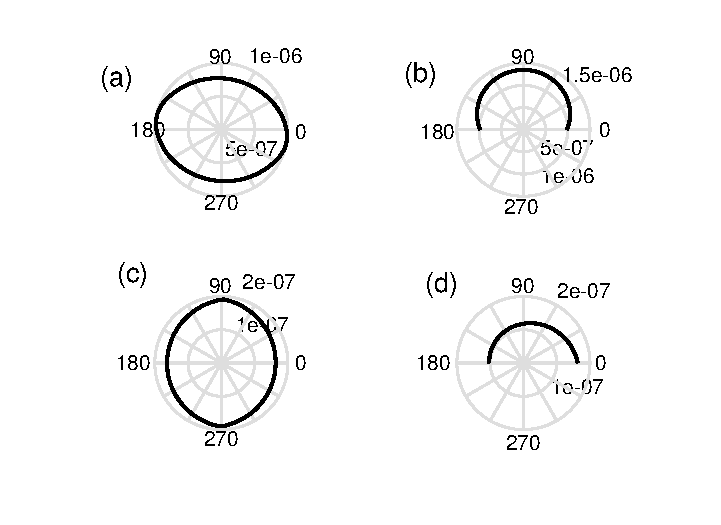
\includegraphics[width=10cm,height=5.3cm]{figures/GC_beamforming/polar1.eps}  
\vspace{-8mm} 
 \caption{\label{fig:polar} Directivity of received signal before (a,b) \& after (c,d) beamforming}
 \vspace{-7mm} 
\end{figure}
  
Note that the maximum transmission power $P^{max}_i$ is limited by the permitted level of signal propagation through tissues as $P_i\leq P_S$. If there are multiple concurrent transmissions, then the cumulative signal at any point should also meet the safety criteria $\sum_{i=0}^{M-1} P_i\leq P_S$. Thus, for safe and energy efficient choice of transmit power, the safety weight is chosen as:
\begin{equation} \label{e:ws}
w_{ij}^s = max\left( \frac{\delta_{jc}^{M-x}}{\hat{\delta}_{j}^{M-x}},\frac{\sum_{i=0}^{M-1} P_i}{P_S} \right),
\end{equation}
$\forall i\in\{1,..,M\}\  \&\  \forall j\in\{1,..,M\} + \{R\}$. Using $w_{ij}^s$, the magnitude of $P_i$ can be estimated using (\ref{eqn:Pi}).
 
\noindent$\bullet$ \textbf{Phase-match weight ($w_{ij}^p$):} As seen in Fig.~\ref{fig:multi}(c), the mismatch in phase among the signals results in destructive signal combination, and thus, reduces the net received power. To perfectly synchronize the uniformly distributed planar implant array, we first match the link-dependent phase shift of each implant obtained in (\ref{e:psi}) with respect to the reference position at ($O$). Then, using the good cross-correlation property of the Gold codes that we use later in Sec.~\ref{sec:cs}, we extract the phase differences from the frequency offsets iteratively as $\gamma' h_{iR}^{M-S}$ and compute the overall phase lag of each implant in the form of Phase match weight as: 
\begin{equation}\label{e:wp}
w_{ij}^p=\psi h_{iR}^{M-S}+\gamma' h_{iR}^{M-S} 
\end{equation}

 \begin{figure*}[t]
	\centering
	%\vspace{-2mm}  %
	\includegraphics[width=17cm]{figures/GC_beamforming/blockDiag.pdf} 
	\caption{\label{fig:spreading} CDMA \& beamforming based MAC framework for implants communication using GC-IBN}
\end{figure*}

\noindent$\bullet$ \textbf{Steering weight ($w^t$):}
This weight allows steering the signal from the transmitter to the relay with the desired beam shape given in Fig.~\ref{fig:polar}.(c)-(d). In the desired beam, along the elevation plane in Fig.~\ref{fig:polar}.(d), the beam power is increased at $\phi$=$0$ towards the position of the relay and in the azimuth plane in Fig.~\ref{fig:polar}.(c), the propagation is steered away from the neighbors at $\theta$=$0,\pi$. The corresponding steering weight is given as: 
\begin{equation} \label{e:wt}
w^{t}_{iR}= sin(k\theta_{iR})cos(k\phi_{iR})+sin(k\theta_{iR})sin(k\phi_{iR})
\end{equation}
where, $\theta_{iR}$ and $\phi_{iR}$ are the respective relative azimuth and elevation angles, respectively, between the implant and relay (refer Fig.\ref{fig:angles}), $k=\frac{2\pi f}{c'}$ is the wave number, $c'$ is the propagation speed of signal through the tissue medium estimated using the permittivity of the medium as,
\begin{equation}
c' = c/\sqrt{\epsilon}\,\, m/s
\end{equation}
where $c$ is propagation speed of light in vacuum and $\epsilon$ is the permittivity of the medium. $c'$ for muscle is around $9.5e6\ m/s$ and that of skin is around $8.3e6\ m/s$.

We adjust the array factor of the $\overrightarrow{H}$ field in (\ref{e:Harray}) using the three weights derived above as, 
\begin{equation}\label{e:AFnew}
E[AF_H]\text{=}\frac{1}{M}\sum_{i=0}^{M-1} \frac{1}{w_{iR}^s} \overrightarrow{H_i}gh_{iR}^{M\text{-}S} e^{j\omega \left(\psi_{iR}^{M\text{-}S}+\gamma_{iR}^{M\text{-}S} \right)} e^{w^{t}_{iR} - w_{iR}^p}
\end{equation}

%\noindent \textbf{Average power pattern \& energy efficiency:}
The average power pattern of the uniformly distributed planar array can be estimated as $E[|AF|] = |AF|(1-\frac{1}{M})+\frac{1}{M}$. 
We use our simulation environment to study the maximum power level in the tissue area using 
\begin{equation}\label{e:Pmax}
P^{max}=max_{\{r,\theta,\phi\}}  E[|AF|]
\end{equation}

\section{Hardware Implementation with Tissue Phantom}
\label{sec:implement}
In this section we implement near-field beamforming developed in section \ref{sec:bf}. We describe the testbed and present the results that quantify the effects of beamforming. 
\subsection{Experimental Setup}

We design a testbed using two USRP X310 software defined radios (SDRs), one each at the transmitter and receiver ends. Two distinct transmitters are installed on the same X310, since the SDR supports up to two LFTX daughter-boards. These low frequency daughterboards are set to 400 KHz center-frequency, which is within the range for galvanic coupling previously identified in~\cite{tbiocas}. Similarly, a LFRX daughter-board is used on the receiving X310. We implement near-field beamforming using the phase-match and steering weights analyzed and calculated in Sec. \ref{sec:bf}. The physical system layout and block diagram are given in Fig~\ref{F:testbed}. We transmit QPSK modulated signals from two transmitters, A \& B simultaneously, with limits on the transmit power to ensure it complies with the ICNIRP rules mentioned in Sec. \ref{sec:exp}.
The SDRs are configured and programmed in MATLAB utilizing the wireless communications toolbox functions.
In order to ensure that there is no ground coupling between the transmitters and the receiver, the receiver is connected to a battery source. All SDRs are given the same external clock inputs through the  OctoClock, also from National Instruments, to ensure synchronization.

\begin{figure*}[h!]
\centering

    \begin{subfigure}[b]{0.35\textwidth}
        \centering
        \includegraphics[width=0.95\linewidth]{figures/GC_beamforming/testbed_labels.jpg}
        %\caption{Physical experimental testbed} 
        \label{F:testbed}
    \end{subfigure}%
    \begin{subfigure}[b]{0.6\textwidth}
        \centering
        \includegraphics[width=0.95\linewidth]{figures/GC_beamforming/testbed_schem.pdf}
        \label{F:testbed}
    \end{subfigure}
    \caption{Photo and diagram of the testbed}
    \label{F:testbed}
\end{figure*}


For the purpose of this testbed, the same data is generated and sent from the two transmitters to ensure a common bit-stream for beamforming. 
Each data set, after modulation, is multiplied by a phase offset to apply its beam weight and achieve constructive interference.
The beam weights for each transmitter is calculated using equations \ref{e:wp} and \ref{e:wt}. The weights are then summed together and applied to the transmitted signal as per (\ref{e:AFnew}). The phase match weight  ($w^p$) is a sum of the phase offset induced by the channel and modeled in \cite{tbiocas} and the frequency offset of the cross-layer path from muscle to fat to skin (M-S).
Even though the entire system is connected on a common 10 MHz clock ensuring hardware frequency synchronization, we note there exists a constant frequency offset, possibly that of the cross-layer path. In our experimental setup we compensated for this effect in the receiver using a MATLAB coarse frequency compensator function. The steering weights ($w^t$) are calculated using the physical distances of the transmitters, from each other and from the receiver.

The transmitting electrodes are placed on the muscle layer. The beam-formed GC signal is received by the receiving electrodes that are placed on the skin layer, acting as the relay node. In the following subsection, we present the results of the received signal strength measurements and BER.

\subsection{Experimental Results}
There is an increase in received signal power when the two transmitters' weights are phase matched. As seen in Fig. \ref{fig:RSSI}, there is an increase of 3 dB in the received power when the two transmitters are in phase from the lowest received power achieved using TX A.
This result matches the theoretical expected doubling in received power with two transmitters. We notice a 1 dB difference between the individual transmissions of the two TXs (A and B). This difference can be attributed in the different paths between each transmitter and the receiver pair.

The phase offset steering weights are calculated based on the position of the transmitters and receiver, thickness of tissue phantom, using (\ref{e:wt}). The steering weight is summed with the phase match weight and is introduced to the transmitter as a phase offset to TX B. However, during experimentation we discovered a range of phase offsets for which the highest received power did not change significantly (more than 0.4 dB). In order to investigate the effect of the phase offset on the received signal strength for a wide range of phase angles, we performed an angle sweep keeping the phase offset of TX A at \ang{0} and varied the phase offset of TX B from \ang{1} to \ang{360}. As the results in Fig. \ref{fig:anglesweep} show, the maximum received power occurs at \ang{87}, whereas for the same setup the theoretical optimal phase offset should be \ang{62}, neglecting the frequency offset $\gamma' h_{iR}^{M-S} $ of equation (\ref{e:wp}). That offset is neglected because of the frequency compensation of our system. We notice that the received signal strength from \ang{60} to \ang{110} does not increase by more than 0.4 dB, ensuring that the constructive interference occurs for a range of approximately \ang{50}. The destructive interference has its lowest point at \ang{270}.

 \begin{figure}[t]
	\centering
	%\vspace{-2mm}  %
	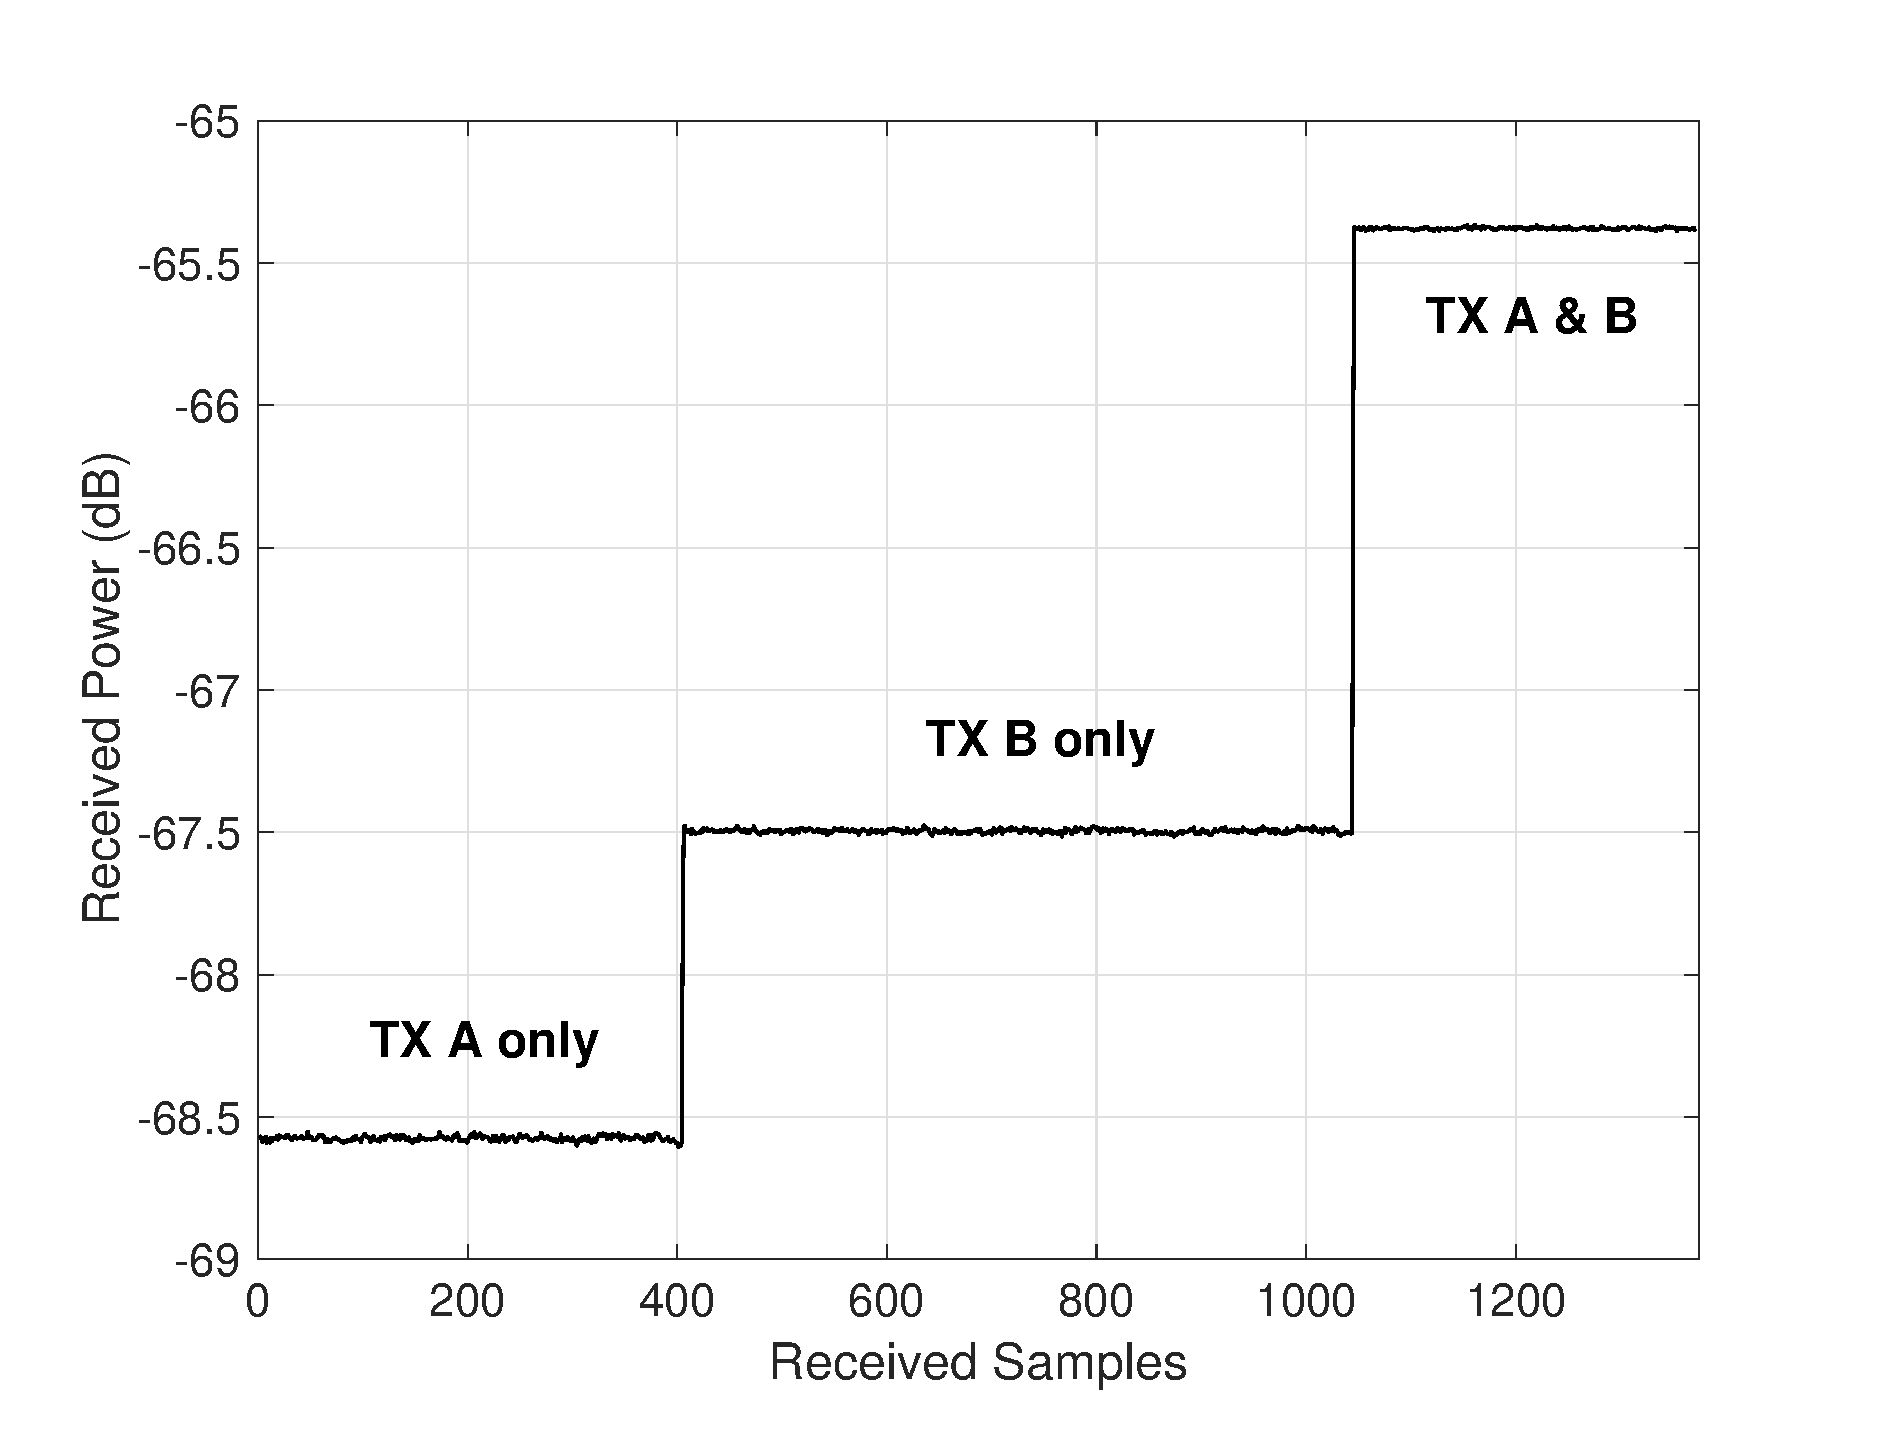
\includegraphics[width=0.7\textwidth]{figures/GC_beamforming//RSSI_curve_80.eps} 
	%\vspace{-3mm}
	\caption{\label{fig:RSSI} Received Signal Strength of three configurations (Tx A only, Tx B only and Tx A \& B) with phase match weights} \vspace{-2mm}
\vspace{-3mm}
\end{figure}

 \begin{figure}[t]
    \centering
	%\vspace{-2mm}  %
	\includegraphics[width=0.7\textwidth]{figures/GC_beamforming/BER_plot_finall.pdf} 
	%\vspace{-3mm}
	\caption{\label{fig:BER} Average BER measurements for 4 configurations (Tx A only, Tx B only, Tx A and B with phase match weights, Tx A and B without phase match weights) }
\vspace{-3mm}
\end{figure}

\begin{figure*}[t!]
\centering

    \begin{subfigure}[b]{0.5\textwidth}
        \centering
        \includegraphics[width=0.95\linewidth]{figures/GC_beamforming/comsol_nobf.png}{a}
        \caption{Logarithmic current density without beamforming} 
        \label{F:nobeamf}
    \end{subfigure}%
    ~
    \begin{subfigure}[b]{0.5\textwidth}
        \centering
        \includegraphics[width=0.95\linewidth]{figures/GC_beamforming/comsol_bf.png}{b}
        \caption{Logarithmic current density with beamforming}
        \label{F:beamf}
    \end{subfigure}
    \caption{COMSOL\textsuperscript{\textregistered} simulations for current density throughout phantom tissue}
    \label{F:comsol}
\end{figure*}

We also simulated the behavior of our setup using the finite element analysis COMSOL software, to measure current density at various points of the skin layer. As seen in Fig. \ref{F:comsol}, when the beamforming weights are applied to the two transmitters, there is higher current density at the receiver. These simulations prove that applying beamforming within our system effectively combines the power of several implants and increases the system efficiency.

Our testbed is designed to study intra-body communication as a whole, by providing insights on the communications front of implanted sensors transmitting measurements to a receiving on-skin relay. For this reason, the decoding capabilities of the system are of great interest. With an increase in received signal strength, and therefore SNR, the BER of the system when beamforming is enabled is lower than that of individual transmissions. As seen in Fig. \ref{fig:BER}, the BER of the system when both transmitters are transmitting with beamforming falls in the order of $4e$-$4$, compared to $2e$-$3$ for the scenario with no beamforming. This proves that an implant network where multiple sensors transmit with matched phases resulting in constructive beamforming results in a system with better decoding capabilities. We performed experiments for both wet and dry conditions and it can be seen that the wet conditions lead to a lower BER overall since the received signal strength improves through wet tissue. The received signal strength of our system does not exceed 0.31 $ \mu W$, which is below the mW range provided in \cite{ICNIRP}, while we also monitor the TX power to ensure safe transmissions.
 \begin{figure}[t]
	\centering
	%\vspace{-2mm}  %
	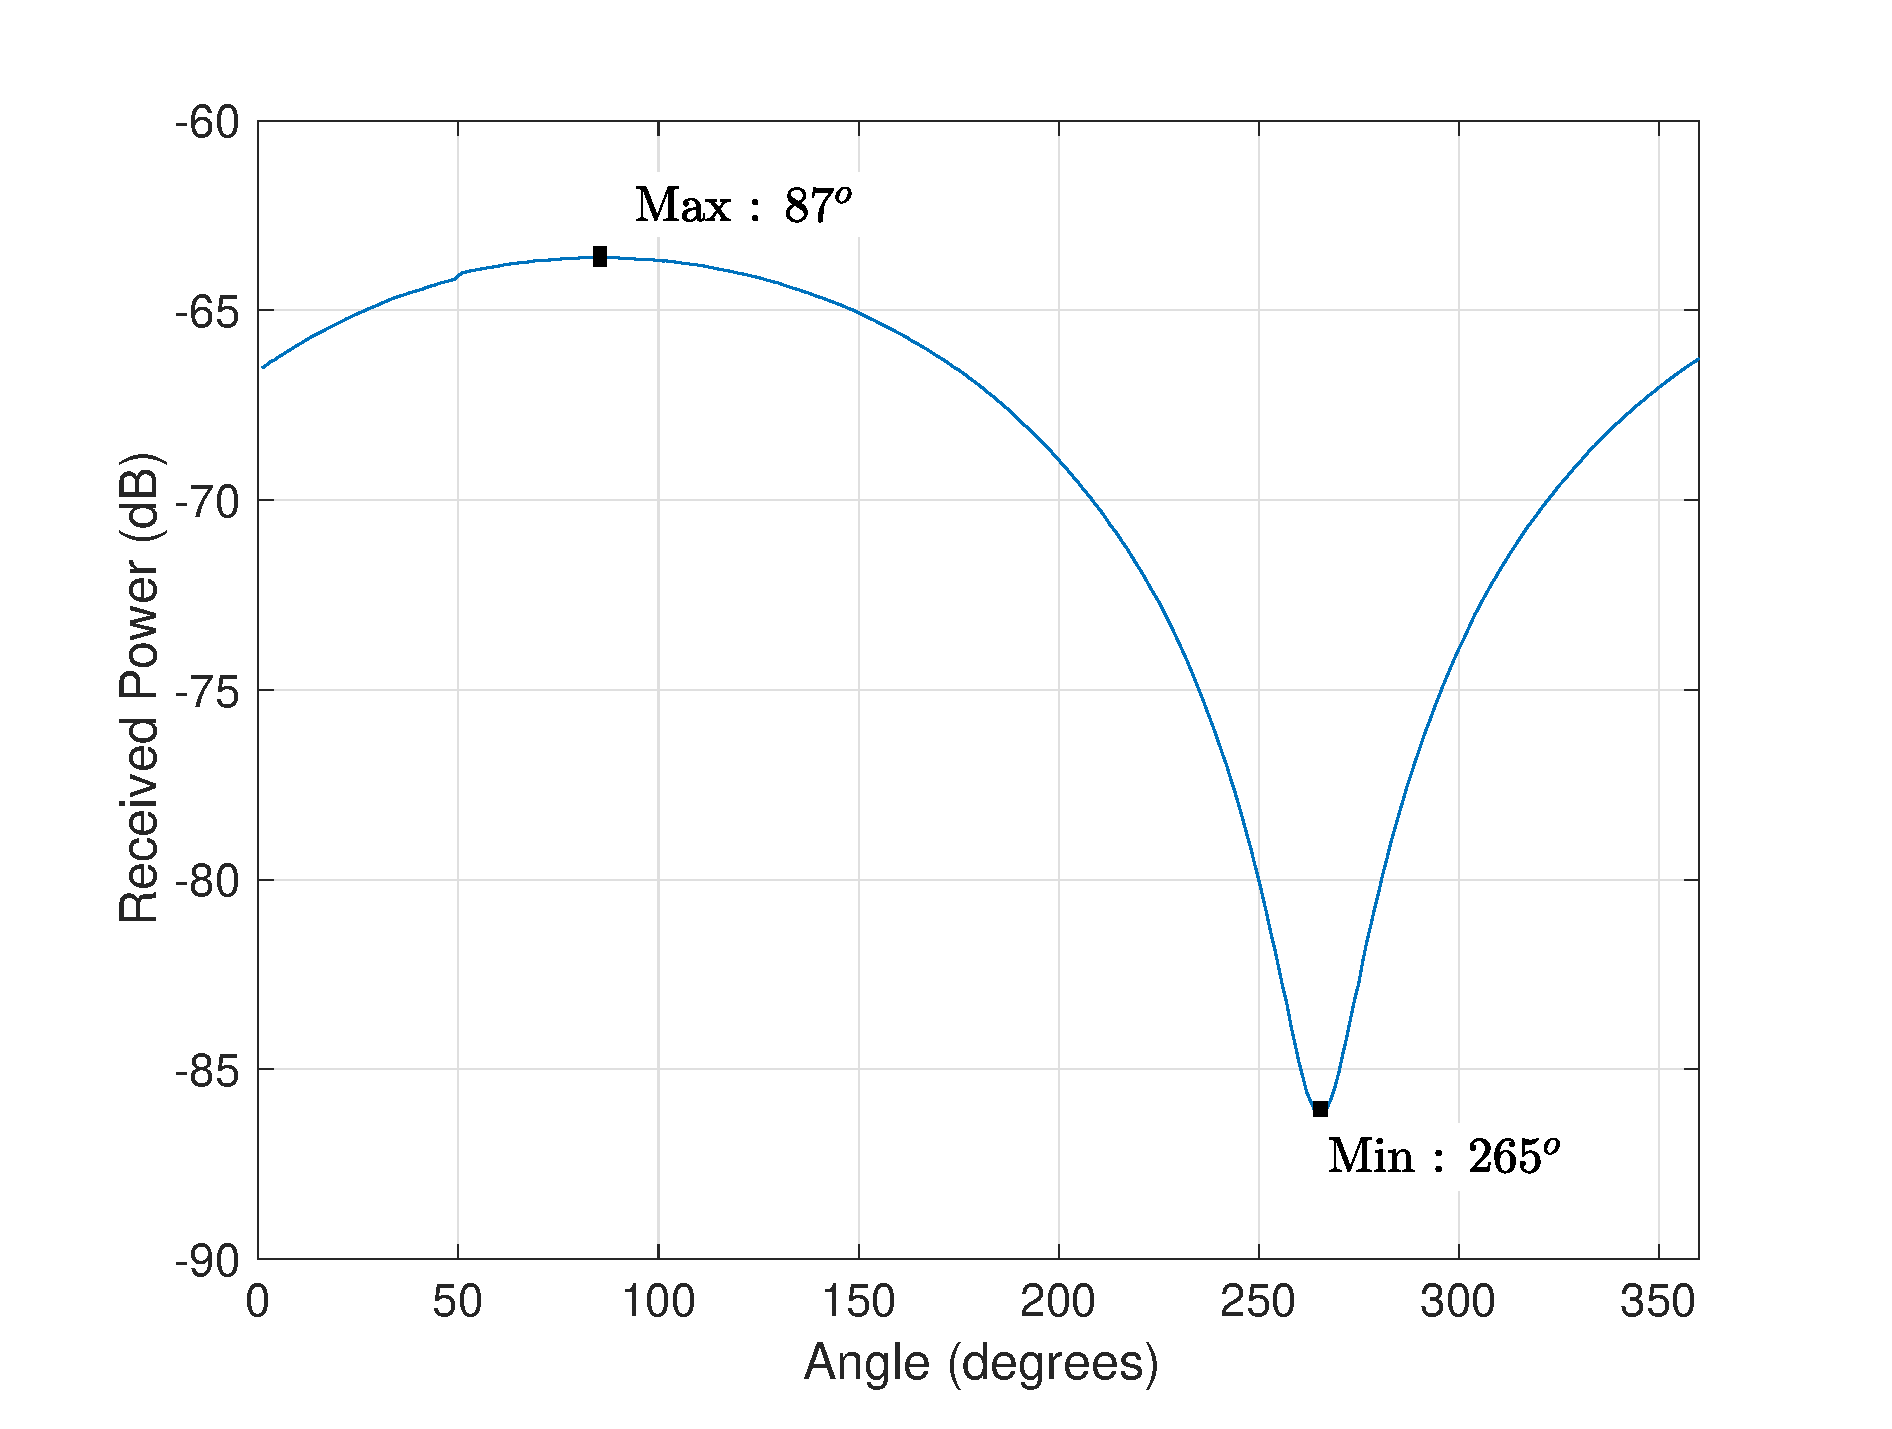
\includegraphics[width=0.95\linewidth]{figures/GC_beamforming/angle_sweep_fig.eps} 
	%\vspace{-3mm}
	\caption{\label{fig:anglesweep} Received Signal Strength with two transmitters, changing the angle of Tx B from 0-360 degrees} \vspace{-2mm}
\vspace{-3mm}
\end{figure}


\section{Beamforming using joint Compressive Sensing-CDMA} 
\label{sec:cs}
Implants participating in distributed beamforming fashion must transmit a common data vector to the on-skin relay. We propose a CDMA procedure to share data among the implants before initiating the beamforming process.
Specifically, we develop a compressive sensing (CS) transmission technique to reduce the number of measurements to send, which further results in lowering the transmission time and energy.	
The beam formation and the process of end-to-end data communication is split into five stages, as described below (see Fig.~\ref{fig:flowchart}):

\noindent $\bullet$ \textbf{Stage I. Resource assignment by the relay:} Each communication cycle starts a parameter setting beacon by the relay that allows implants to synchronize, set duty cycles for peerlevel and beamforming-based communication, use CDMA codes to partition the collision domain, and compute feedback weights for the array factor given in (11), (12) and (13) for optimal beamshaping (refer to stage.1 in Fig.10). Communication from implants are acknowledged in a successive round, enabling the implants to sleep immediately after they transmit the beam. Specifically, the parameters setting includes a synchronization message that delivers the information about two synchronization time slots. In the first time slot window the implants are allowed to send their data to a peer aggregator, while during the second time slot all the implants listen for the collected data that the aggregator is sending back to them. At the end of the second time slot, each implant sends such common data to the relay on the surface acting as distributed beamforming. Such procedure is required since we need each implant to have a common data vector prior to beamforming, thus the relay also appoints an aggregator (IDA) for the communication round. The aggregator’s role is simply to collect the individual and simultaneously transmitted spreaded sequences that combine in the tissue channel, and save this as the common data vector. The aggregator is a peer-implant, and its role is rotated in every round. Note that only a coarse synchronization is required during peer communication phase as specified at Stage III: an implant can choose to transmit anytime within the allowed window. For this purpose, quasi-orthogonal CDMA Gold codes are chosen for their good performance in an asynchronous CDMA transmissions.

%Before the implants share their data through the CDMA scheme, a precoding CS scheme is employed at each implant in order to send less samples of data
Specifically, a joint CS-CDMA scheme is proposed where the Gold codes are multiplied by the CS coding matrix. This way, the implants send less samples of data to further save energy while exploiting the possibility of fast simultaneous transmissions. Both the decoding and decompression of data are performed only at the on-skin relay, so that the implants do not have to perform any complex tasks.

\noindent $\bullet$ \textbf{Stage II. CS downsampling of data transmission:}
CS theory allows to reconstruct a signal with much lower samples than its dimension, provided that signal is sparse in some basis \cite{CDSP} and restricted isometric property (RIP) is satisfied \cite{candes} \cite{Vizziello}. Following this reasoning, implants may send a lower amount of sensed data reducing the energy consumption, one of the main concern in intra-body networks.\\
In practical applications, implants may not transmit data continuously. Hence, we assume that the sensed data is sparse, i.e., the implant activity is sporadic and i.i.d with probability $p_a\ll 1$ in the considered time window.
Thus, the sensed data $\mathbf{b}_i$ of size $U \times 1$ at implant $m_i$ may be 
represented as a linear measurement $\mathbf{x}_i$ of size $N \times 1$ with $N\ll U$ as
\begin{equation}
{\mathbf{x}_i=\mathbf{F}_i \mathbf{b}_i}
\label{eqCS}
\end{equation}
that corresponds to CS coding matrix multiplication block in the left side of Fig. \ref{fig:spreading}, where measurement vector $\mathbf{x}_i$ is a compressed version of $\mathbf{b}_i$ obtained through the CS coding matrix $\mathbf{F}_i$, i. e., the dictionary, with
\begin{equation}
\mathbf{F}_i=\mathbf{Q}_i \mathbf{\tilde{F}}_i 
\label{eqCDMA2}
\end{equation}
where the elements of $\mathbf{\tilde{F}}_i$ are taken from Rademacher distribution and $\mathbf{Q}_i$ is the discrete Fourier transform (DFT) matrix. 
Note that  $ \mathbf{b}_i \in \mathcal{B}_{a}$, where $\mathcal{B}_{a}$ is the discrete alphabet $\mathcal{B}$ augmented to represent also the inactivity. Specifically, an inactive implant is equivalent to transmit symbol $0$ while  activity corresponds to data modulated according to the alphabet $\mathcal{B}$ \cite{Dekorsy12}.\\ 
The size of the compressed data $\mathbf{x}_i$ that implant $m_i$ shares through the CDMA procedure is much lower than the original $\mathbf{b}_i$.
Moreover, since the transmission for some health applications is sporadic and also short, we can interpret it as  group sporadic transmission, which allows to develop a faster CS algorithm as detailed in Stage V.

\noindent $\bullet$ \textbf{Stage III. Peer communication phase:} The relay provides a time window ($T_B$) for all implants to combine their data using the Gold codes and transmit them simultaneously. 
Note that an implant can opt out of transmission in a cycle and sleep for prolonged period if its sensing cycle is longer. Also, the communication is not strictly synchronized that relieves the implants from complex scheduling and mutual phase offset computation for this first round of messaging. An implant can choose to transmit anytime between the allowed window of peer-level communication.
This transmission is intentionally set to very low power given that it traverses the high-gain M-M path to the aggregator node (refer to stage.2 in Fig.\ref{fig:flowchart}).The spreading factor $L$ of the Gold code is chosen based on the number of implants. The implant ID is associated with a unique spreading code sequence $\mathbf{c}_i$ within the CDMA codebook.\\ 
For $N$ compressed data bits $\mathbf{x}_i$ of the implant $i$, each
bit is directly multiplied by the Gold code $\mathbf{c}_i$ with $L$ elements to generate the spread sequence $x_{i,n}\mathbf{c}_i,\ \forall \ i\in\{1,..,M\},\  n\in\{1,..,N\}$ of size $L\times 1$ (refer to the Gold code generator multiplication in  Fig. \ref{fig:spreading}). These quasi-orthogonal Gold codes have good cross correlation properties that enable simultaneous almost non-interfering transmissions. After spreading at the sampling time instant corresponding to the index $k,\ \forall k \in \{0,..,L-1\}$, the implants transmit the spreaded sequence $x_i\mathbf{c}_i$ through the M-M path. At this stage, neither other implants nor the aggregator performs any decoding. 

 
At $n$-th bit time instant, the aggregator receives the sequence $\mathbf{d}_n$ as a vector of size $L \times 1$ from the $M-1$ implants as,
\begin{equation}
	\mathbf{d}_n = \sum_{i=1}^{M-1} g_{iA}^{(M-M)} x_{i,n} \mathbf{c}_i  + \mathbf{w} 
	\label{eqCDMA0}
\end{equation}

where $A$ represents the aggregator, $x_{i,n}$ is the $n$-th bit sent by the implant $m_i$ after applying CS,  $\mathbf{c}_i=[c_i(0), c_i(1),..., c_i(L-1)]^T$ is the spreading code for implant $m_i$ with $x_{i,n} \mathbf{c}_i$ expressed in antipodal form, $()^T$ denotes the transpose, and 
$\mathbf{w}$ is the iid additive white Gaussian noise vector with zero mean and variance $\sigma^2$ of size $L \times 1$ given by $[w(k-L+1), w(k-L+2),..., w(k)]^T$. Since each implant transmits in a narrow band channel ($400\ kHz$) the M-M channel can be represented as a single tap channel \cite{tbiocas}. We assume that $g_{ij}^{(M-M)}$ is constant during a transmission cycle. 

The final vector $\mathbf{d}$ of size $LN \times 1$ is given by
\begin{equation}
	\mathbf{d} = [\mathbf{d}_1 \phantom{x} \mathbf{d}_2 \phantom{x} ... \phantom{x} \mathbf{d}_n \phantom{x} ... \phantom{x} \mathbf{d}_N] 
	\label{eqCDMAd}
	\end{equation}
Eq. (\ref{eqCS})-(\ref{eqCDMAd}) summarize the joint CS-CDMA procedure for data transmission, showing that the sent data $\mathbf{d}$ is given by the original bits $\mathbf{b}_i$ for each implant $m_i$ in (\ref{eqCS}) multiplied by a combination of CS coding matrix $\mathbf{F}_i$ and Gold codes $\mathbf{c}_i$.\\
 
Once the aggregator receives the overall CDMA vector containing the spread data $\mathbf{d}$, it sends back the common CDMA vector $\mathbf{d}$ representing the aggregated value to the peer implants through a single broadcast, again using the high-gain M-M path. 

The spread data received back at the $m_i$-th implant can be expressed as
\begin{equation}
\tilde{\mathbf{d}}_i=g_{Ai}^{(M-M)}\mathbf{d} + \mathbf{w}
\label{eqCDMA2b}
\end{equation}
Now, all the implants have the common CDMA vector (refer to $\tilde{\mathbf{d}}$ in Fig. \ref{fig:spreading}), which may only slightly differ from each other depending on the channel coefficient of the M-M path from the aggregator to the specific implant according to (\ref{eqCDMA2b}).
  
\begin{figure}
 \centering
% \vspace{-2mm}  %
\includegraphics[width=8cm,height=11cm]{figures/GC_beamforming/diagram.pdf}  
\vspace{-2mm} 
 \caption{\label{fig:flowchart} Stages showing the entire end-to-end implant to relay communication}
 \vspace{-6mm}
\end{figure}
   
\noindent $\bullet$ \textbf{ Stage IV. M-S Beamforming phase:}
In this phase, each implant acts as an independent antenna array element and attempts to form a beam sending the same overall CDMA data vector that has been shared with all the implants at the instant $T_B$ predetermined by relay. The use of the same CDMA data during beamforming further improves the  SNR and lowers the required M-S transmission power at the implants as shown in Sec.\ref{sec:bf}. Although each implant acts as an element of a virtual antenna array sending the same information, the individual implant signals differ in amplitude and phase, as instructed by the beamforming weights. The implants tune their transmission based on the weights, such that all the transmissions from implants constructively amplify the received signal $\mathbf{y}$ at the relay and maximize the received power.

Thus, each implant sends the information at lower power compared to individual transmissions in the M-S channel, enabling significant energy savings.The received vector $\mathbf{y}$ at the relay (as shown in Fig. \ref{fig:spreading}) is given by
\begin{equation}
	\mathbf{y}=\sum_{i=0}^{M-1} S_{i} \tilde{\mathbf{d}}_i + \mathbf{w}
	\label{eqCDMA3}
\end{equation}
where $S_{i}$=$\frac{1}{w_{iR}^sM}gh_{iR}^{M\text{-}S}e^{j\omega\left(\psi_{iR}^{M\text{-}S}+\gamma_{iR}^{M\text{-}S} \right)} e^{w^{t}_{iR} - w_{iR}^p}$ obtained from (\ref{e:AFnew}) that accounts for both the steering coefficient of the implant $m_i$ and the channel coefficient of the M-S path from the implant implant $m_i$ to the relay $R$ on surface. The implants enter into the sleep state immediately after sending the beam until the next transmission cycle (see stage.3 in Fig.~\ref{fig:flowchart}).

\begin{figure*}[t]
 \centering
 \vspace{-2mm}  %
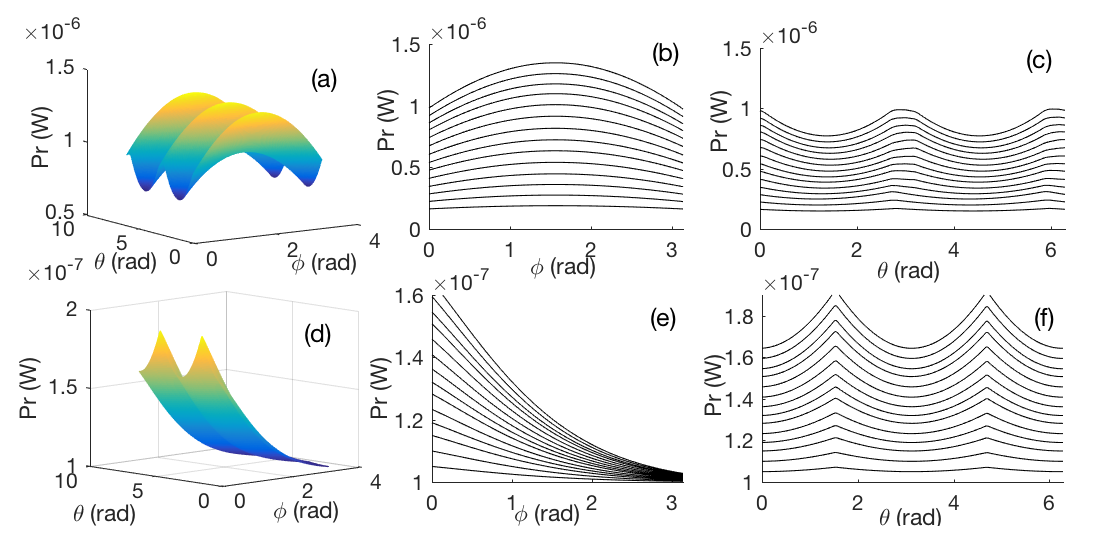
\includegraphics[width=17cm,height=6.5cm]{figures/GC_beamforming/multi.eps}  
 \caption{\label{fig:multi} Received power before and after beamforming}
 \vspace{-5mm}
  \end{figure*}
  
\noindent $\bullet$ \textbf{Stage V. Despreading, decoding and feedback at the relay:}

Having received the common CDMA vector through the beamformed signal, the relay performs despreading and CS data reconstruction using a matrix with the same Gold codes distributed to the individual implants and the CS coding matrices. In this way, it recovers the sensed data and the associated ID of each implant, as shown in the Relay block in Fig. \ref{fig:spreading}.\\ 

Going in more details, CS methods can be categorized broadly into accurate and stable convex relaxation iterative algorithms \cite{Donoho06}, \cite{Candes08}, and fast but less accurate greedy algorithms \cite{Masood13}, \cite{Dai09}. Since health applications require high reliability we focus on an accurate iterative solution. Specifically, as said before, in such applications the implant activity may be interpreted as group sporadic, thus we develop a group basic pursuit denoising (Group-BPDN) approach to reconstruct the sent data $\mathbf{b}_i$.
The  problem may be expressed as \cite{BergFriedlander:2008}
\begin{equation}
	\textrm{min} \    \  \sum_{v=1}^V\|\mathbf{b}_{i,v} \|_2   \ \textrm{  subject to } \|\mathbf{F}_i\mathbf{b}_i-\hat{\mathbf{x}}_{i} \|_2 \le \sigma
	\label{eqCSgroup}
\end{equation}
where the index $v$ refers to the group to which the data have been assigned, $\mathbf{F}_{i}$, $\mathbf{b}_{i}$, $\mathbf{x}_{i}$ are defined in (\ref{eqCS}), and $\sigma$ is the noise variance. The estimate  $\hat{\mathbf{x}}_{i} = [\hat{x}_{i,1} \phantom{x} \hat{x}_{i,2} \phantom{x} ... \phantom{x} \hat{x}_{i,n} \phantom{x} ... \phantom{x} \hat{x}_{i,N}]$ of size $N \times 1$ is obtained through the CDMA despreading that uses the cross-correlation of the received signal $\mathbf{y}$ in (\ref{eqCDMA3}) with the known Gold codes. 
Specifically, the element $\hat{x}_{i,n}$ of $\hat{\mathbf{x}}_{i}$ is calculated as
\begin{equation}
\hat{x}_{i,n}=\mathbf{y}^T_n\mathbf{c}_i
\label{eqCDMA4b}
\end{equation}
where $\mathbf{y}_n$ is the $L \times 1$ element of the $LN \times 1$ vector $\mathbf{y} = [\mathbf{y}_1 \phantom{x} \mathbf{y}_2 \phantom{x} ... \phantom{x} \mathbf{y}_n \phantom{x} ... \phantom{x} \mathbf{y}_N]$ and $()^T$ indicates the transpose.
\\
Note that the Group-BPDN minimizes quadratic
noise by solving the convex optimization
problem as a quadratic programming approach for which
efficient Interior-Point (IP) methods exist \cite{BergFriedlander:2008},
\cite{berg2}.


In terms of transmission and propagation time, the whole transmission cycle takes 
\begin{equation}\label{time}
4\displaystyle \frac{L}{\eta}\text{+} 2\frac{\psi x_{iR}^{M\text{-}M}+\gamma x_{iR}^{M\text{-}M}}{360 f}\text{+} 2\frac{\psi x_{iR}^{M\text{-}S}+\gamma x_{iR}^{M-S}}{360 f}\text{+}4T_R 
\end{equation} seconds, where $L$ is the frame (or chip) length and $T_R$ is the tissue relaxation time required between transmissions to assure normal tissue temperature under abnormal blood flow rates, calculated as $T_R= \sqrt{\frac{\epsilon}{\sigma}}$, $\epsilon\  \& \  \sigma$ being the tissue permittivity and conductivity.  

Finally the relay computes the weights $w^s_{iR}$,$w^p_{iR}$ and $w^t_{iR}$ using (\ref{e:ws}), (\ref{e:wp}) and (\ref{e:wt}) for the successive transmission and transmits them to the implants at the predetermined interval as given in the Beamforming weights block in Fig. \ref{fig:spreading} and in stage.1 in Fig.~\ref{fig:flowchart}.




\section{Performance Evaluation \& Results}\label{sec:results}   

In this section, we evaluate the energy savings achieved by the proposed CDMA based beamforming framework by (i) analyzing the proportion of energy propagating in the direction of the relay to that leaking in the undesired directions, (ii) studying the influence of the number of array elements on the implant power consumption, (iii) quantitatively measuring the improvement in implant lifetime, and (iv) comparing the energy consumption for the overall M-S path communication with/without our approach. We develop a 3-D multi-layer, heterogeneous tissue channel model in MATLAB, operating at a narrow band of $100\ kHz$. The tissue area has the dimension of $20\times 20 \mathrm{cm}$, with $r_{max}$=$20\ \mathrm{cm}$. The separation between the layer of implants in muscle and the surface is $2.2\ \mathrm{cm}$. The maximum safe transmit power is $1\ \mathrm{mW}$.

 \begin{figure}[b]
 \centering
\vspace{-6mm} 
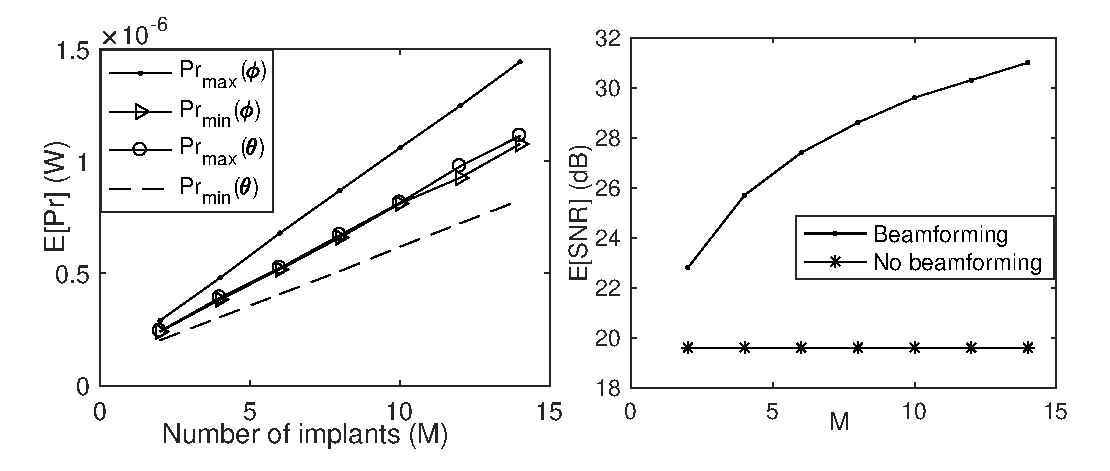
\includegraphics[width=0.95\textwidth]{figures/GC_beamforming/new2plots.eps} 
\vspace{2mm} 
 \caption{\label{fig:prplot} (a) Directionality (b) SNR before \& after beamforming} 
  \end{figure}
  
\subsection{Effectiveness of beamforming} The pattern of received power at the relay resulting from the sum of the signals concurrently propagating through the tissue medium without beamforming is shown in
Fig.~\ref{fig:multi}(a)-(c). Here, the propagation is oriented towards the longitudinal muscle direction (at $\phi$=$\frac{\pi}{2}$, $\theta$=$0,\pi$), where more energy flow occurs along the length of the arm. This causes minimal flux at the surface relay (at transverse direction at $\phi$=$0$). This pattern may also cause more interference to the potentially neighboring implants (refer Fig.~\ref{fig:expr}(left) for the direction of neighbors). Before beamforming, the ratio of energy flow in the required direction to undesired direction is $\approx 0.53$. Fig.~\ref{fig:multi}(d)-(f) shows the received signal at relay after beamforming, where more power is steered towards the relay (at $\phi$=$0$) and there is less power in the longitudinal direction ($\phi$=$\frac{\pi}{2}$, $\theta=0,\pi$) mitigating the interference to neighbors. 

Fig.~\ref{fig:multi}(b)-(c) shows power degradation when signals with different phases are combined together. After the phase mismatch is rectified using $W^p$ in the beamforming process, the signals add up constructively (refer Fig.~\ref{fig:multi}(e)-(f)) as demonstrated in Fig.~\ref{fig:expr}(d) and improve the received power by an additional $\approx 3\%$ as shown in Table.\ref{tab:result1} as $Pr(W^p)$. Note that this is the received power obtained after the transmit power is reduced to sufficient level using $w^s$ weight.
 We analyze the maximum induced power at every point in the given tissue area defined by $\theta$, $\phi$ and $r$ using (\ref{e:Pmax}) and verify that the cumulative received power at any point in the tissue with multiple concurrent transmissions does not exceed the restrictions posed by safety limits, confirming the tissue safety and normal thermal distributions~\cite{ICNIRP}. Using the simulation environment, we further ensure that $\int_{\theta} \int_{\phi} \int_{r} Pr dr d\phi d\theta \leq 25\ \frac{mA}{m^2}$. 

\noindent \textbf{Influence of number of implants:}
The resulting proportion of power in the required to undesired direction is plotted in Fig.~\ref{fig:prplot}.(a) illustrating that more power is steered towards the relay when there are more number of implants forming the array. Thus both the critical beamforming parameters namely, the per implant power conservation and the directivity of beamforming, are improved with the number of implants or array elements ($M$). The actual SNR for individual transmission from each implant through M-S path is compared with the exponential increase in SNR at the receiver after beamforming with $M$ implants in Fig.~\ref{fig:prplot}(b). 


\noindent \textbf{Implant lifetime:}
The transmission power of the implants is reduced to just meet the required SNR by applying the safe weight $w^s$ derived in (\ref{e:ws}). The resulting power consumed ($aPt$) in each implant vs $M$ and the corresponding improvement in implant lifetime is shown in Table.\ref{tab:result1}. %KRC- is the vs M or N? 
We see that the implant life dramatically extends from $10$ weeks when used without beamforming, to $\approx 138$ weeks with beamforming for the scenario with $14$ implants.	
  
\begin{figure}
	\centering
	%	\includegraphics[width=1\linewidth]{gbp_ber1.eps}
	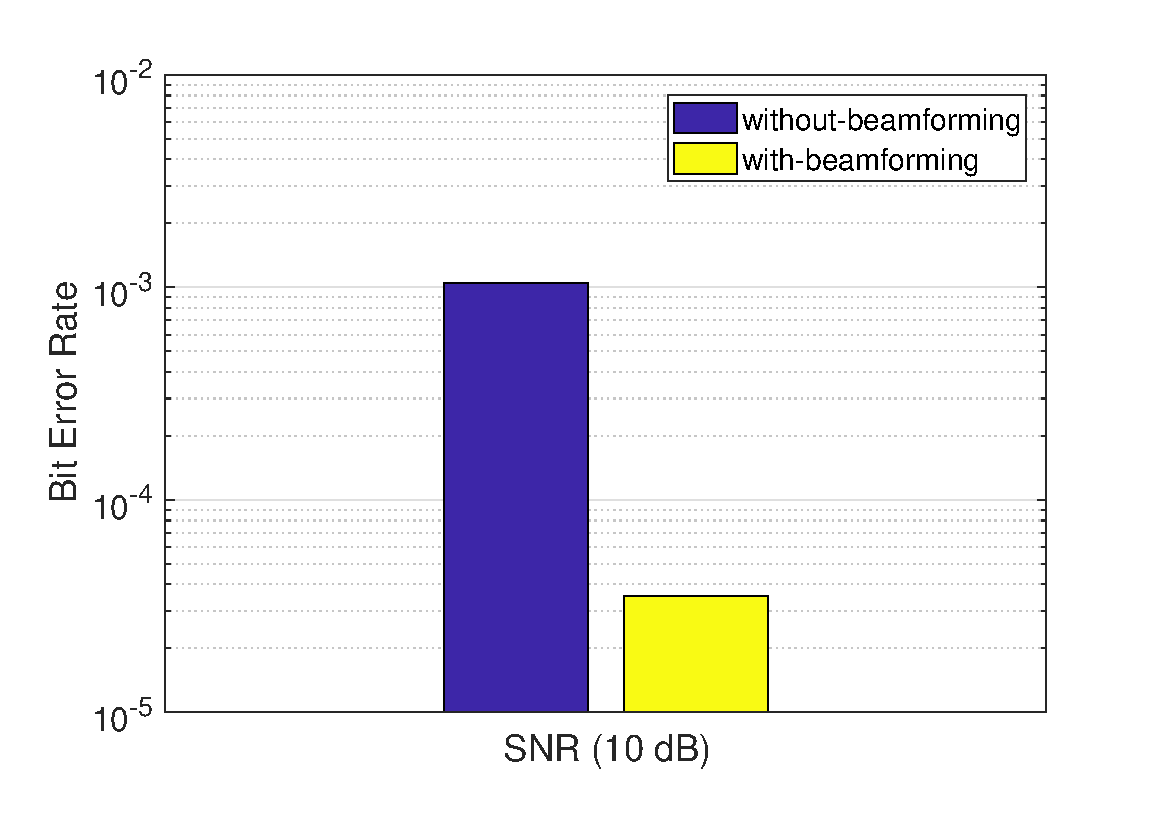
\includegraphics[width=10.5cm,height=7.5cm]{figures/GC_beamforming/sensor2delay2_beamforming_bar.eps}
	\caption{Bit error rate for CS-CDMA solution based on Group-BPDN and Gold codes with and without beamforming. Spreading sequence $L = 128$ chips, sparsity $= 40 \%$, maximum delay $= 2$ chip time duration, number of implants $M = 2$, data length $U = 5000$, compressed measurements $N = 2500$.}
	\label{Fig_result0}
	\vspace{-2mm}
\end{figure}

\begin{figure}[h!]
\centering
    \begin{subfigure}[b]{0.95\textwidth}
    	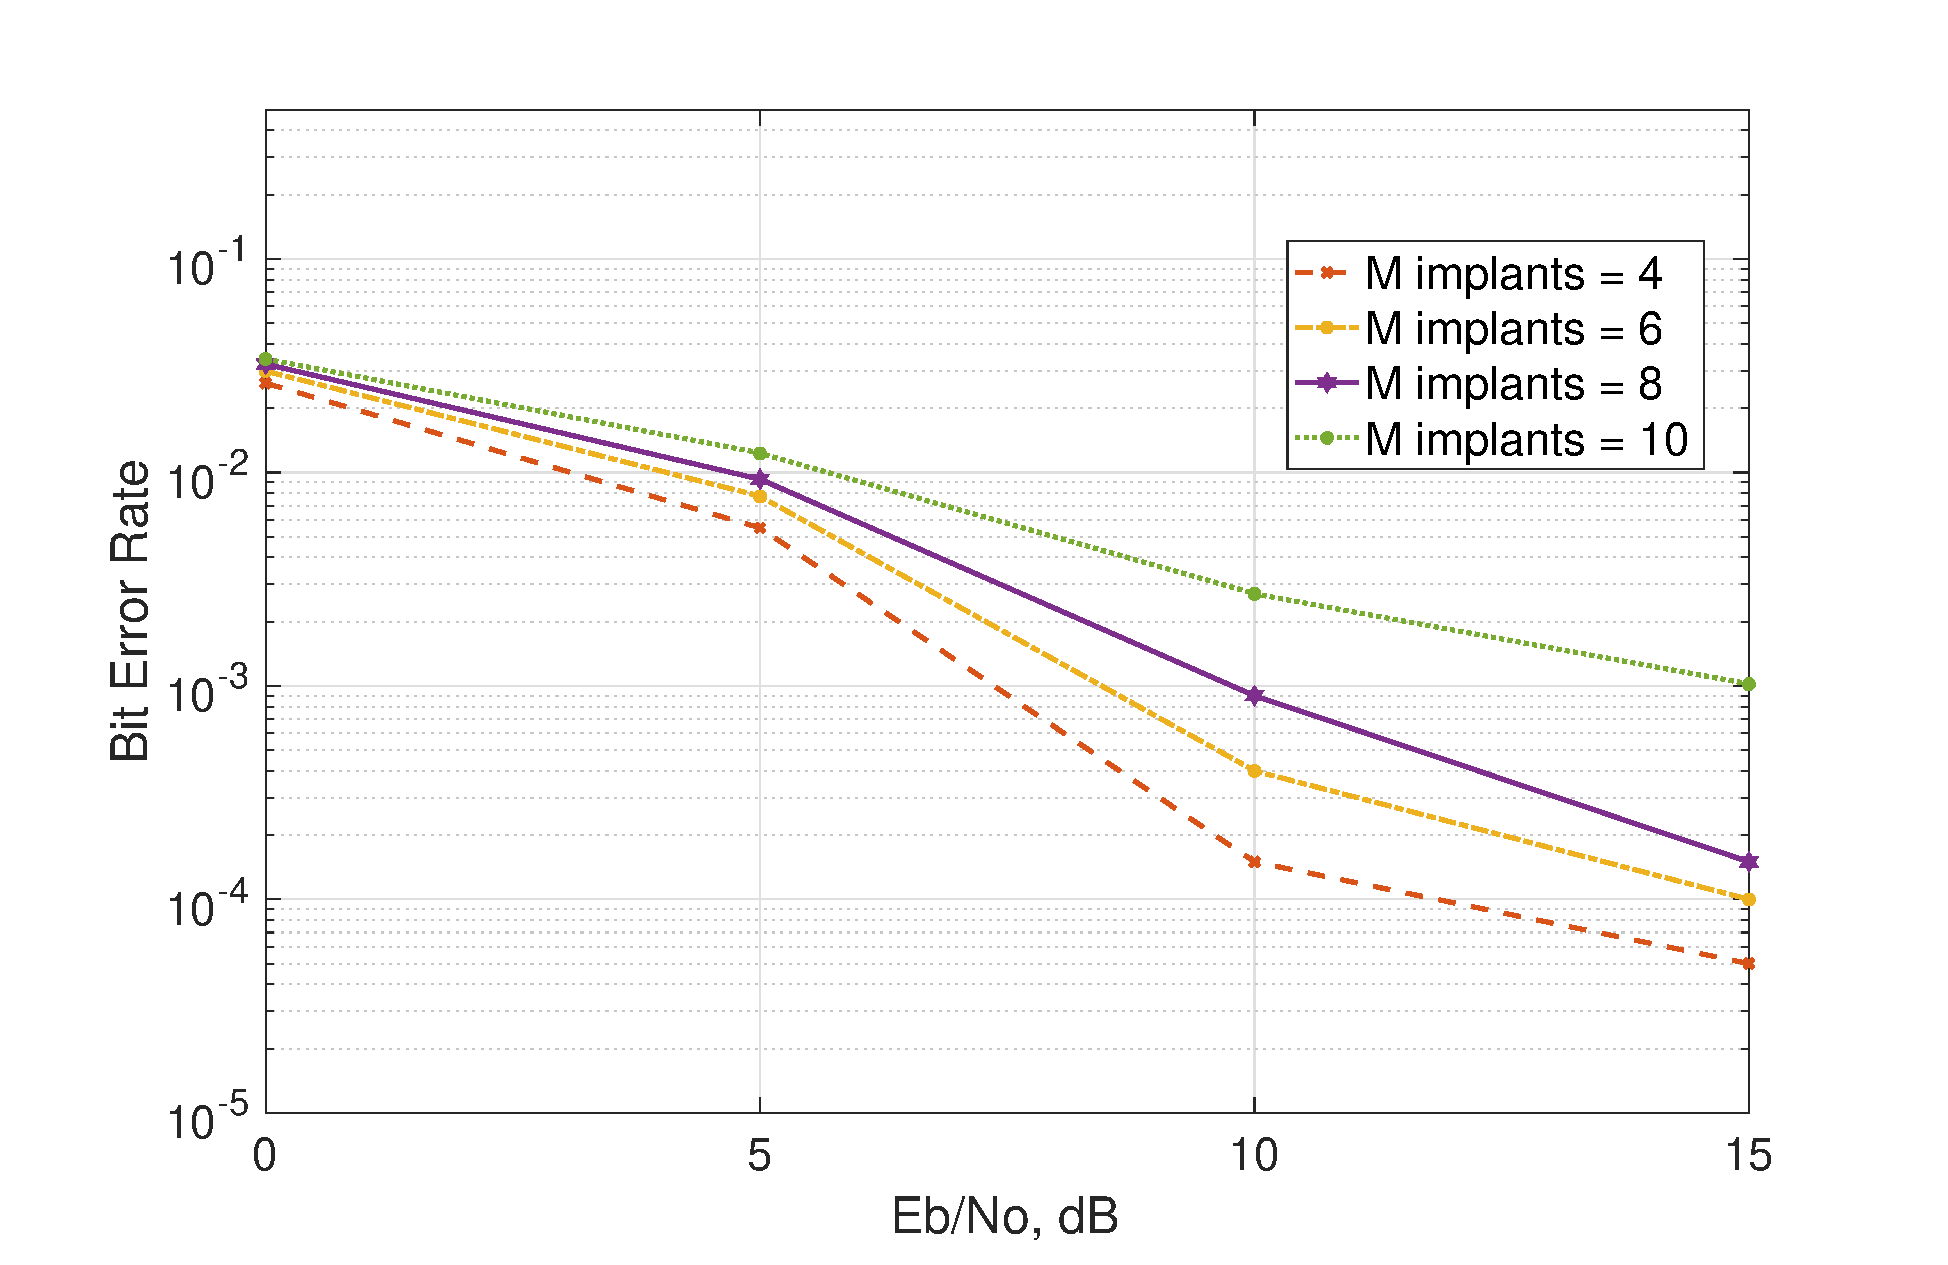
\includegraphics[width=\textwidth]{figures/GC_beamforming/ber_sensors_sp-40-delay_2.eps}
    	\caption{BER for CS-CDMA solution based on Group-BPDN and Gold codes, maximum delay $= 2$ chip time duration}
    	\label{Fig_result1}
    \end{subfigure}
    ~
    \begin{subfigure}[b]{0.95\textwidth}
	    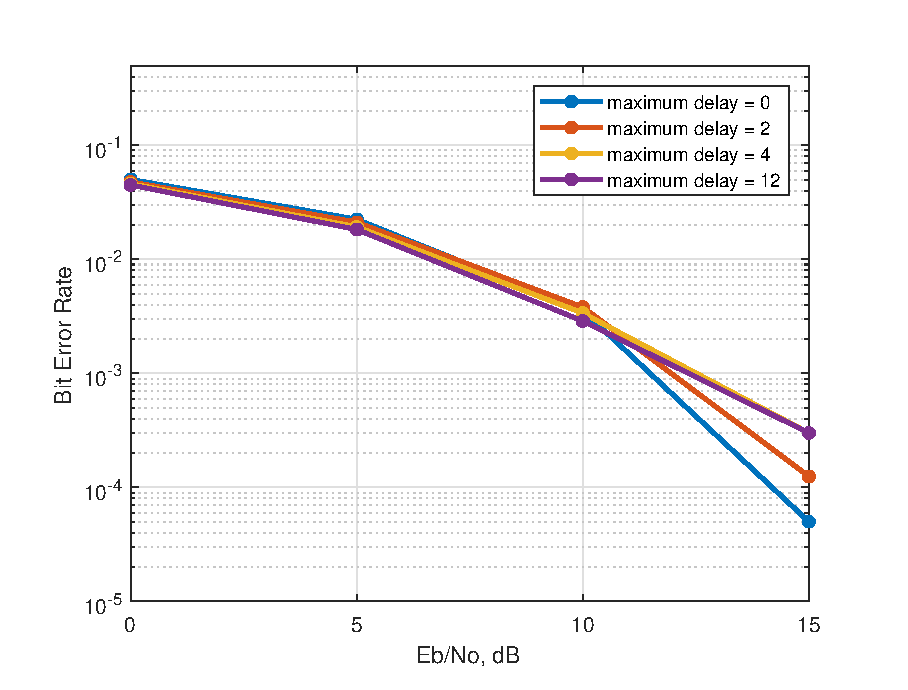
\includegraphics[width=\textwidth]{figures/GC_beamforming/delay_sp-40-sen-8.eps}
	    \caption{BER for CS-CDMA solution varying the max. delay (\# of chips) among implants' transmissions of the asynchronous scheme}
    	\label{Fig_result1bis}
    \end{subfigure}
    \caption{BER of CS-CDMA. Spreading sequence $L = 128$ chips, sparsity $= 40 \%$, data length $U = 5000$, compressed measurements $N = 2500$}
    \label{F:CSCDMABER}
    \vspace{-3mm}
\end{figure} 
  
\subsection{BER \& energy analysis for CS-CDMA beamforming}

The proposed CS-CDMA scheme allows concurrent transmissions for the implants which reduces the total time for data transmission. The implants perform only simple tasks to send the acquired data, while the burden despreading/decoding is carried out only at on-skin relay. Moreover, the CS procedure allows to further reduce the transmission time since a much lower number of samples are sent instead of the full senses data. There is, however, an additional overhead of (i) spreading the data using the Gold codes, and (ii) (albeit high gain M-M) communication between implants to the aggregator and back. We aim to study whether this cost is offset by the energy savings achieved by beamforming.

The proposed algorithm for asynchronous CS-CDMA recovers both the activity of the implants and their data in a certain time window.
The total number of sensors varies between $2$ and $10$. The spreading factor $L$ for the Gold codes is set equal to $128$ and the Group BPDN CS approach is used to recover data with different level of sparsity, which corresponds to the percentage of implant's activity in a certain time window.

Fig. \ref{Fig_result0} shows a comparison between the BER achieved by the proposed CS-CDMA solution with and without beamforming under the same parameter setting of the experimental setup in Sec. \ref{sec:implement}. Specifically two implants are considered and the BER improvement is due to SNR gain (2.5 dB) obtained when using beamforming.

The simulation results on Fig. \ref{Fig_result1} compare the achieved BER for different number of implants, describing that the system shows good performance with an increased number of implants. Fig. \ref{Fig_result1bis} illustrates the BER performance versus the maximum delay among the implant's transmissions. Each implant transmits with a random delay within the maximum one to simulate the asynchronous scheme in the peer communication phase inside the muscle. In low $E_b/N_0$ region the performance for different delays is comparable, while lower delays give better results when increasing $E_b/N_0$.

Fig. \ref{Fig_result2} focuses on the choice of the dictionary matrix $\mathbf{F}_i$ in (\ref{eqCDMA2}) for the proposed CS-CDMA algorithm. Indeed, the design of such matrix is one of the main concern in CS algorithms for an efficient solution. We compare the proposed $\mathbf{F}_i$ definition, based on DFT and rademacher distribution, with only DFT, and Gaussian and Bernoulli random matrix. The total amount of measurements has been fixed to $5000$ and results in Fig. \ref{Fig_result2} prove that the proposed solution shows high performance even when sending only $50 \%$ measurements, differently from DFT, Gaussian and Bernoulli matrices.

Fig. \ref{Fig_result3} compares the accuracy of the proposed CS-CDMA solution, based on Group-BPDN CS approach, with a modified version of it, i.e., when employing the greedy regularized group orthogonal matching pursuit (ReGOMP) algorithm. Fig. \ref{Fig_result3} shows that the proposed Group-BPDN based approach outperforms the ReGOMP solution for both values of sparsity ($20 \%$ and $40 \%$), showing high accuracy already when sending only $50 \%$ measurements. Note that for health applications the high accuracy is a stringent requirement.

\begin{figure}
	\centering
	%	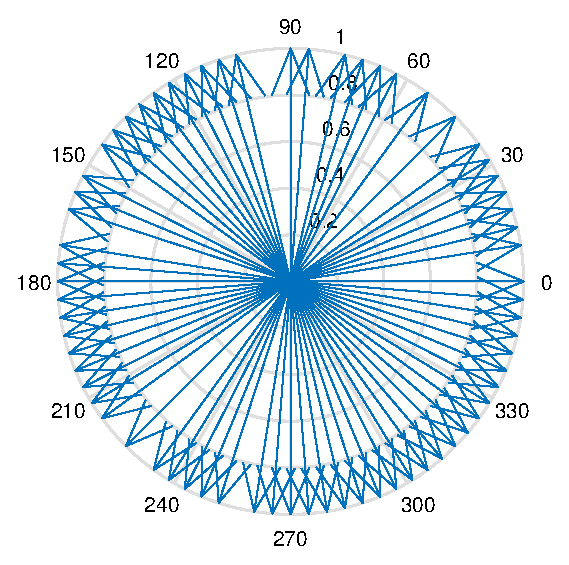
\includegraphics[width=1\linewidth]{dict_angles.eps}
	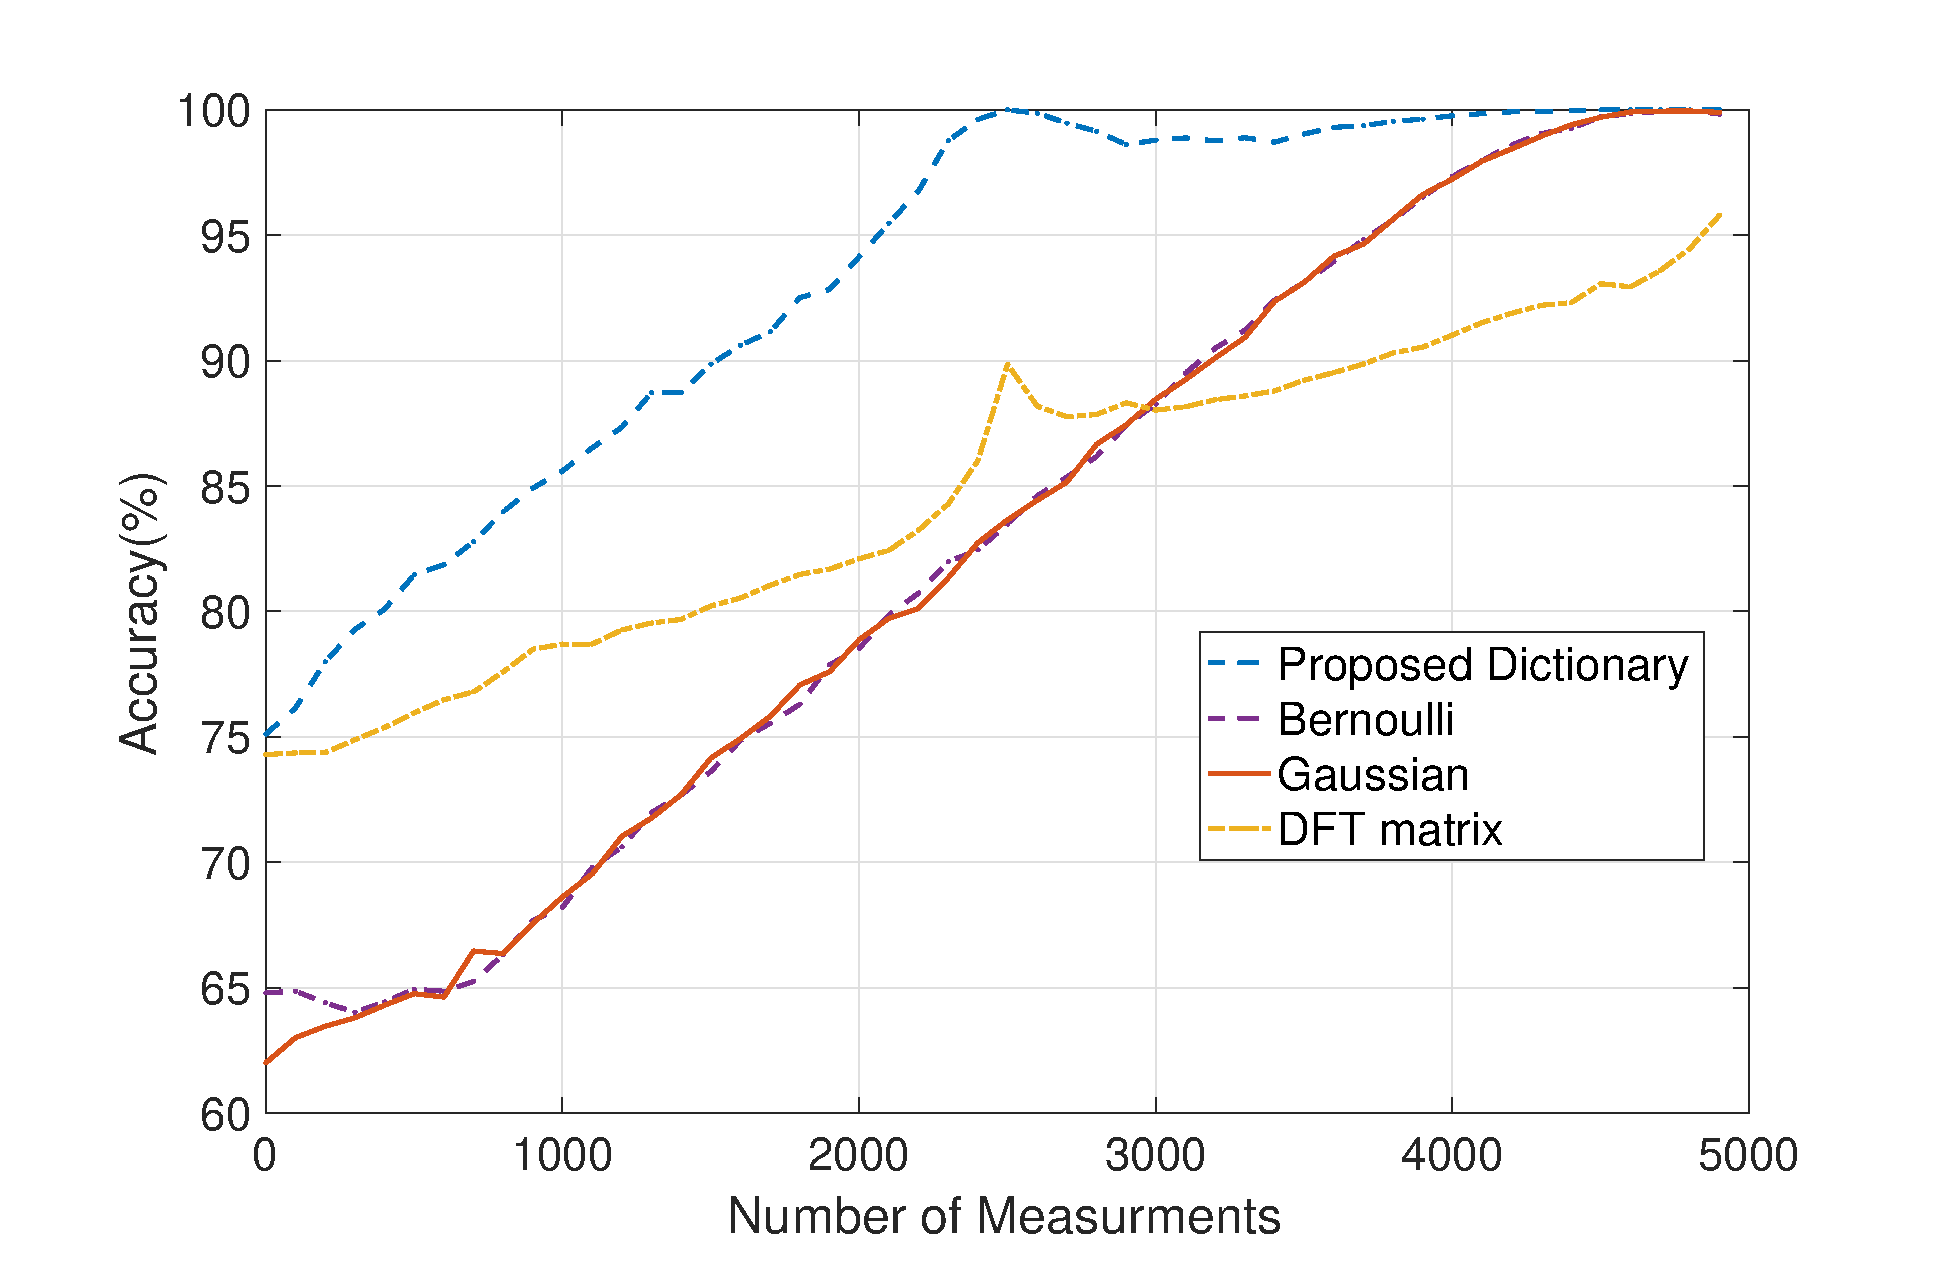
\includegraphics[width=0.95\textwidth]{figures/GC_beamforming/sen4sparsity-50-delay2-1.eps}
	\caption{Accuracy of the proposed CS-CDMA algorithm for different CS coding matrices.}	
	\label{Fig_result2}
\end{figure}
\begin{figure}
	\centering
	%	\includegraphics[width=1\linewidth]{dif.eps}
	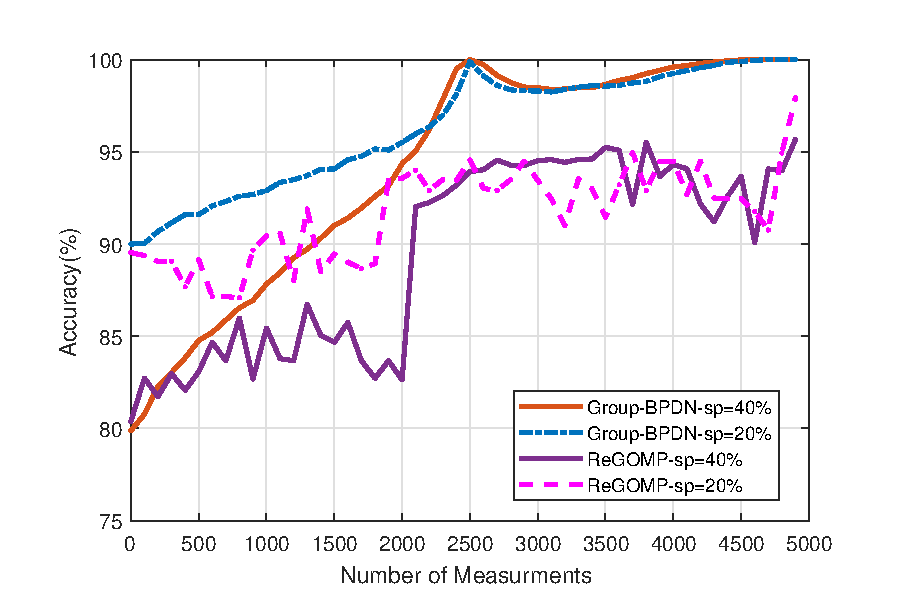
\includegraphics[width=0.95\textwidth]{figures/GC_beamforming/measuremDelay2sen4.eps}
	\caption{Comparison betweeen the proposed CS-CDMA scheme based on Group-BPDN and its modified version using ReGOMP. Maximum delay $= 2$ chip time duration, sparsity (sp) $= 20 \%$ and $= 40 \%$.}	
	\label{Fig_result3}
\end{figure}

\noindent \textbf{Network traffic and time:} With the proposed framework with  $L$=$64$, the total traffic flow in a transmission cycle becomes $32$ bytes, which is much lower than the existing IEEE 802.15.6 standard that requires a minimum of $13\times 4$ bytes as frame header alone not including the data. The time required for the whole transmission cycle
%with less transmission rate and tissue breathing time
is estimated using (\ref{time}) for $T_R$=$10\ \mu s$ and $\eta$=$100\ kbps$ to be only $1.3\ ms$ that is mainly dominated by the transmission time.



\noindent \textbf{With and without beamforming:} We next compare the energy consumption for the implant to relay communication through the M-S path with and without the beamforming. For an expected link length of $5\  cm$, the average M-S path-loss is $41.2\ dB$. The energy per bit required for a desired SNR of $\hat{\delta}$ is given using (\ref{eqn:Ptmin}) by $E_b$=$P_i^{min}/\eta$.   
For $\hat{\delta}$=$10$, a noise factor ($N_o$) of $1e$-$8$, data rate $\eta$ of $10 \ kbps$ and bandwidth $\triangle f$ being $1e5\  Hz$,  the required energy per bit ($E_b$) becomes $6.62\ \mu J$. This would allow battery of capacity of $240\ mAh$ to last for $2.89$ years. 
  
Before beamforming, the implants first broadcast their individual codewords in the M-M path. This step requires an energy of $0.68\ \mu J$, considering the same values as assumed above for all other parameters, other than the lower path loss through M-M path ($19\  dB$). The aggregated codeword is then transmitted from the aggregator as a broadcast to all implants that requires $\approx 0.7\mu J$. Finally, the beamforming towards the relay in undertaken in the M-S path, where each node spends about $4e$-$5M^{-1.03}$ times less energy than that actually required for the direct M-S path. For a scenario with 4 implants, the power consumption in each implants for the complete transmission cycle is $1.39\  \mu J$, which is $4.7$ times lower than that required for M-S communication without beamforming. The proposed framework extends the life of implant upto $13.8$ years assuming every other parameter remains the same.


\section{Conclusion}\label{sec:concl}
In this paper, we propose and implement an energy efficient implant to surface relay communication using galvanic coupling and beamforming. The proposed communication technique is strongly focused on improving energy efficiency by: sharing sensed updates among peer-implants using compressed sending CDMA through the high-gain M-M path, avoiding unpredictable data delivery conditions caused by collisions and transmission back-offs. Then, through near-field beamforming performed by the implants organized into distributed transmitter arrays, communication through the vertical tissue layers is achieved with high SNR (or conversely, lower energy per implant). The proposed framework dramatically lowers the net energy required for end-to-end implant to relay communication that is 79\% more energy efficient than the direct case, and extends the lifetime of implants upto $13$ years, while ensuring accurate, low BER communication.
\section*{Acknowledgement}
This material is based on the work supported by the U.S.
National Science Foundation under Grant No. CNS-1740907.




